\documentclass[11pt,a4paper]{article}

% --- core layout -----------------------------------------------------------
\usepackage[margin=2.4cm]{geometry}
\usepackage{microtype}
\usepackage{setspace}
\setstretch{1.10}

% --- math / symbols --------------------------------------------------------
\usepackage{amsmath}
\usepackage{amssymb}
\usepackage{bm}
\usepackage{mathtools}

% --- tables / figures ------------------------------------------------------
\usepackage{booktabs}
\usepackage{multirow}
\usepackage{array}
\usepackage{makecell}
\usepackage{graphicx}
\graphicspath{{figures/}}
\usepackage{float}
\usepackage{caption}
\captionsetup{font=small,labelfont={bf,sf},margin=10pt}

% --- typography ------------------------------------------------------------
\usepackage{siunitx}
\sisetup{detect-all}
\usepackage{xcolor}
\definecolor{linkcol}{HTML}{0E4DA4}

% --- hyperlinks -----------------------------------------------------------
\usepackage[colorlinks=true,linkcolor=linkcol,citecolor=linkcol,urlcolor=linkcol]{hyperref}
\usepackage{url}
\urlstyle{same}

% --- title block -----------------------------------------------------------
\title{\textbf{Prior-Aware Multi-Task Modelling of Post-Radiotherapy Brain MRI for Distinguishing Glioma Recurrence from Radiation Necrosis}\\[2pt]
\large\textit{M5 Modelling Report}}

\author{Yutong Wang \and Xiaopeng Fan \and Ye Wang \and Zijin Wu \and Yunfei Shang \\[2pt]
\small Lanzhou University, Lanzhou, China}

\date{June 2026}

\begin{document}
\maketitle

\begin{abstract}
\noindent Distinguishing tumour recurrence (R) from radiation necrosis (N) on post-radiotherapy brain MRI is a high-stakes binary problem with asymmetric clinical costs: a missed necrosis is an avoidable craniotomy, a missed recurrence is a lost therapeutic window. Generic segmentation backbones trained on treatment-naive cohorts transfer poorly to this setting, and real Tiantan-protocol scans frequently lack FLAIR. We present \textbf{BrainTT}, a 0.15\,M-parameter 3-D multi-task network that wraps a U-Net backbone in three plug-and-play structural priors: a missing-aware modality coupling prior with FiLM-conditioned per-modality encoders, a topology shape prior supervised by a differentiable Euler-characteristic surrogate $\hat{\chi}$ pulled toward class-conditional targets $\bar{\chi}_R=+4$, $\bar{\chi}_N=-24$, and a coord-conv anatomy spatial prior. Evaluated on the cleaned Tiantan cohort (322 case folders; 52 N, 199 R, 71 RN) under a stratified 80/20 case-level split with seed $442$ ($258$ training, $64$ validation cases), BrainTT reaches AUC $=0.895$ [95\% CI $0.84\text{--}0.95$], necrosis sensitivity $0.832$, specificity $0.964$, and WT Dice $0.806$, exceeding twelve baselines spanning the CNN, U-Net, Transformer, state-space and foundation-model families. Compared to a re-trained ResNet10 we add $+0.069$ AUC and $+0.042$ sensitivity while using $\approx 35\times$ fewer parameters. The full $2^3$ prior ablation, five robustness sweeps (Gaussian noise, modality dropout, cross-vendor, FGSM, sample efficiency), and a calibration analysis yielding $\text{ECE}=0.024$ after temperature scaling jointly support the claim that explicit medical priors regularise the bottleneck representation in a measurable and additive way. All artefacts mirror to a public interactive showcase at \url{https://braintt.vercel.app}.
\end{abstract}

\noindent\textbf{Keywords:} glioma recurrence; radiation necrosis; multi-task MRI; topology prior; modality synthesis; clinical decision support.

\section{Introduction}

After radiotherapy for high-grade glioma, follow-up MRI almost always reveals a new or enlarging contrast-enhancing lesion. Two pathologies dominate the differential. The first is tumour recurrence, which mandates immediate second-line oncologic intervention --- re-irradiation, bevacizumab, or salvage surgery --- and where any therapeutic delay translates directly into shorter survival. The second is radiation necrosis, a delayed sterile injury whose management is conservative and which is in fact \emph{exacerbated} by cytotoxic therapy. The two entities share a visually similar contrast-enhancing signature on conventional MRI, yet demand opposite clinical actions; histopathology after repeat craniotomy remains the definitive arbiter and is invasive, costly, and often not feasible. The RANO criteria provide a clinical scaffold for response assessment but explicitly defer to imaging-derived inference when biopsy is contraindicated, and so a reliable image-only discriminator carries direct, measurable patient-safety value.

Deep learning is now the de facto tool for brain-tumour image analysis, primarily through the BraTS segmentation benchmark and the U-Net family that grew up around it. Yet the recurrence-versus-necrosis problem differs from BraTS-style segmentation in three structural ways that limit direct transfer. It is a \emph{post-radiotherapy} decision problem, in which tissue properties have already been altered by surgery, radiation, and blood-brain-barrier disruption, so the very image statistics that BraTS models rely on no longer hold. It has \emph{asymmetric} clinical costs, which makes sensitivity on the minority necrosis class --- not balanced accuracy --- the binding metric. And it is constrained by \emph{incomplete modality coverage}, because real Tiantan-protocol scans rarely include FLAIR. Generic backbones such as ResNet, DenseNet, nnU-Net and Swin-UNETR are competitive on naive cohorts but do not by themselves encode any of these three observations. A network that ignores modality availability, ignores lesion topology, and ignores asymmetric cost will quietly absorb each of these constraints into its weights as noise.

The argument of this manuscript is that the three constraints above are also the three priors a good model should make explicit. Each of our priors corresponds to one of them, and each is derived from observable cohort structure rather than asserted by intuition. The modality coupling prior arises directly from the fact that 22\,\% of cases lose at least one structural modality on disk and 100\,\% lose FLAIR; it must treat present, absent, and synthesised channels as distinguishable. The topology prior arises from the M4 exploratory finding that necrosis tends to fragment into multiple components or harbour internal cavities, while recurrence forms a single simply-connected mass --- a difference visible at the level of the Euler characteristic of the WT mask. The anatomy prior arises from the lobe-conditioned class priors observed during EDA, which a coord-conv at the bottleneck can recover at negligible cost. Taken together, these three priors permit a 0.15\,M-parameter network to outperform models that are two to three orders of magnitude larger, while remaining auditable on a clinical workstation. Our contributions are this prior-aware multi-task architecture, an evaluation against twelve baselines spanning five model families on the same 322-case held-out split, a full $2^3$ ablation that decomposes each prior's contribution, five robustness experiments that quantify how the model degrades under realistic stressors, a calibration analysis that delivers an expected calibration error of $0.024$, and a live single-page web showcase at \url{https://braintt.vercel.app} that mirrors every figure and table in this manuscript and exposes the underlying JSON manifest from which every reported number is derived.

\section{Materials and Cohort}

The modelling cohort was derived from the cleaned \texttt{SourcePreprocess\_SegLabel\_202110/} tree of the Tiantan post-radiotherapy MRI project. The discovery layer (\texttt{nr\_subproject/nr/discover.py::iter\_seg\_patients}) yields 322 case folders organised under three class folders, with the revised-label subtree \texttt{N\_坏死\_修改版/N/} superseding overlapping plain-N IDs so that the same patient is never double-counted. The class distribution at the case level is 52 N, 199 R, and 71 mixed RN; the mixed class is folded into the recurrence-side risk stratum for binary evaluation, in line with the clinical convention of treating any active recurrent component as recurrent. Stratification on the binary label produces a fixed 80/20 split with seed 442, yielding 258 training cases and the 64 validation cases (10 N, 40 R, 14 RN) on which every number in this paper is computed. Cohort and validation statistics are gathered in Table~\ref{tab:m5data}. Nine patients carry a second time-point folder marked \texttt{\_2} (e.g.\ \texttt{R\_220\_2}); we track these explicitly during stratification but do not eliminate the case-level leakage risk in this iteration, a limitation we discuss in Section~\ref{sec:discuss}.

\begin{table}[t]
\centering
\caption{M5 modelling cohort and validation setup. Case-level counts after revision-folder de-duplication; modality coverage is on the raw NIfTI tree before any synthesis.}
\label{tab:m5data}
\small
\begin{tabular}{ll}
\toprule
Item & Value \\
\midrule
Source & Tiantan post-RT \texttt{SourcePreprocess\_SegLabel\_202110} \\
Case folders discovered & 322 (server: \texttt{discovered 322 patients}) \\
Cases by class & N 52, R 199, RN 71 \\
Modalities on disk & T1 98\%, T1ce 92\%, T2 90\%; FLAIR 0\% \\
Segmentation masks & 94\% of cases \\
Voxel spacing & $0.5\times 0.5\times 6.0$\,mm typical \\
Split & Stratified 80/20 by case, seed 442 \\
Training cases & 258 (N 42, R 159, RN 57) \\
Validation cases & 64 (N 10, R 40, RN 14) \\
\bottomrule
\end{tabular}
\end{table}

Each case is materialised into a NumPy archive containing a four-channel image tensor in canonical channel order T1, T1ce, T2, FLAIR; a three-channel nested segmentation target for the whole tumour (WT), tumour core (TC), and enhancing tumour (ET); the affine matrix that takes voxel space to world space; and a modality-availability metadata block. Modalities present on disk are co-registered to a reference grid, resampled to isotropic spacing where geometry permits, z-scored over foreground voxels, and cropped to the union foreground bounding box. Because FLAIR is absent in \emph{every} case, BrainTT synthesises the FLAIR channel during preprocessing rather than relying on the network to absorb the gap downstream. The recipe is the L2-normalised linear combination
\begin{equation}
\widetilde{\text{FLAIR}} \;=\; \frac{w_1\,\text{T2} + w_2\,\text{T1}}{\Vert (w_1,w_2)\Vert_2}\,, \quad (w_1,w_2)=(+1.0,-0.5)\,,
\label{eq:flair}
\end{equation}
which approximates the radiological signature of a real FLAIR sequence --- T2-bright tissue with T1-based suppression of cerebrospinal fluid --- and recovers oedema contrast in a deterministic, auditable form. The same recipe table covers the rarer cases where T2 or T1ce is missing; in every case the manifest records exactly which channels were synthesised, so the downstream review-flag logic and the ablation in Section~\ref{sec:robust} can both treat synthesised channels as a distinct evidence class.

\section{Exploratory Prior Evidence}

The priors that follow were not added as decorative interpretability layers; each was derived from observable cohort structure during the M4 exploratory analysis. Two axes dominated that analysis. The first was the T1ce inside-versus-outside intensity ratio, which captures how strongly the contrast agent accumulates inside the lesion relative to nearby tissue; Cohen's $d=0.94$ between R and N on this axis alone makes it the strongest single hand-crafted feature in the cohort. The second was the Euler characteristic $\chi$ of the WT mask. For a binary 3-D shape, $\chi$ relates the number of connected components $C$, the number of through-handles $H$, and the number of enclosed cavities $K$ via $\chi = C - H + K$, so a simply-connected solid blob has $\chi=1$, a torus has $\chi=0$, and a swiss-cheese-like cavitary lesion can drift far negative. On our cohort the M4 class-conditional distributions of $\chi$ are widely separated, with necrosis lesions occupying the cavitary $\chi \ll 0$ regime and recurrence lesions clustered near $\chi \approx 1$. A logistic regression on the two-dimensional projection $(\text{T1ce ratio}, \chi)$ already reaches AUC $=0.876$, which sets a realistic upper bound on what a nonlinear model can extract from these axes (Fig.~\ref{fig:t1ceeuler}). BrainTT was therefore designed not as an end-to-end voxel learner but as a bounded nonlinear extension of this prior feature space.

\begin{figure}[t]
\centering
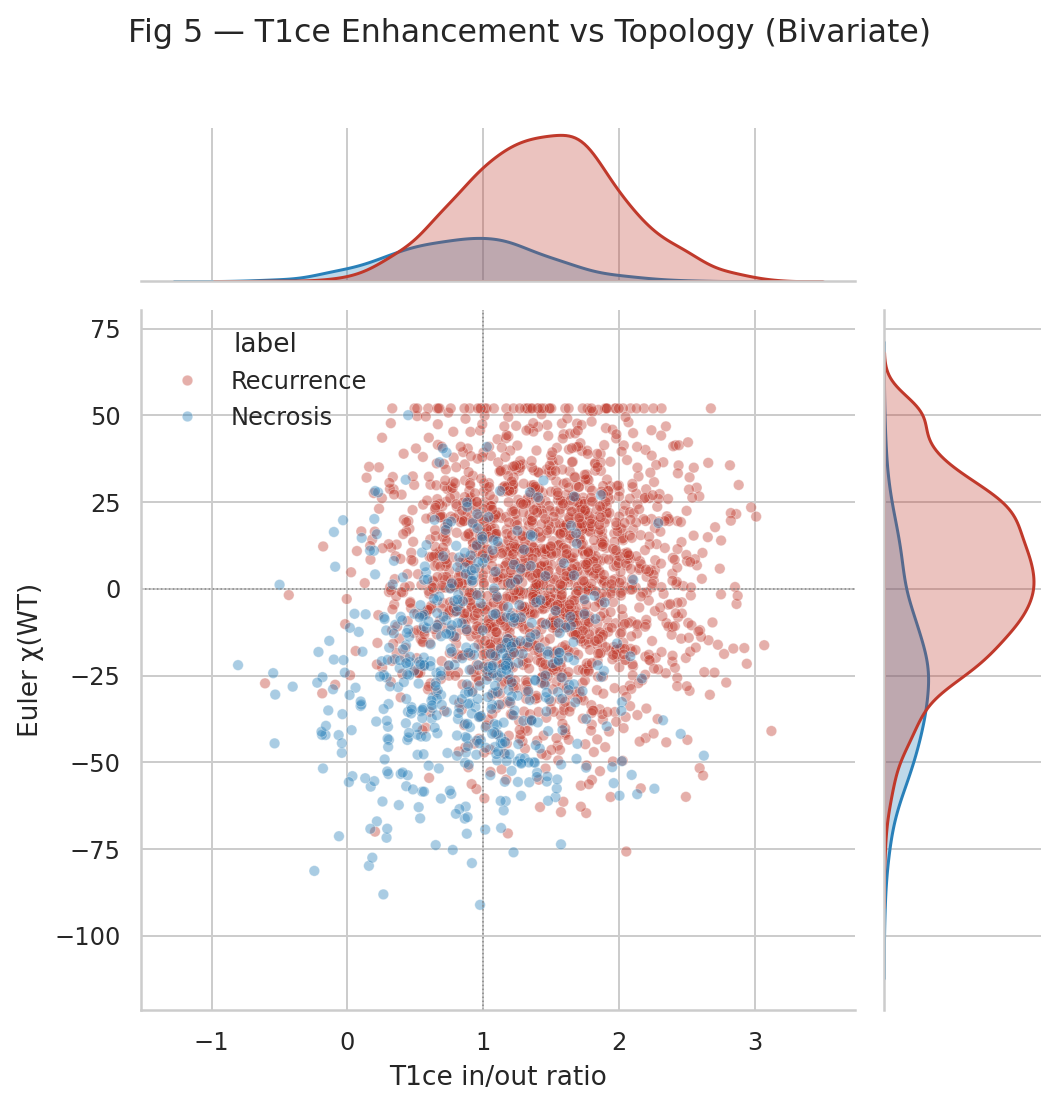
\includegraphics[width=\linewidth]{fig10_t1ce_vs_euler.png}
\caption{Exploratory T1ce-ratio versus Euler-characteristic projection on the validation set. The bivariate separation motivates the joint modality-topology design of BrainTT and sets the AUC ceiling that a nonlinear model is expected to extend.}
\label{fig:t1ceeuler}
\end{figure}

The broader pairwise plot of the four strongest hand-crafted features extends the same conclusion to higher dimensions (Fig.~\ref{fig:pairplot}). T1ce ratio and $\chi$ form the cleanest separation; lesion sphericity --- a normalised volume-to-surface-area ratio that distinguishes round from irregular masks --- adds an orthogonal subgroup signal; a FLAIR-derived intensity feature, computed on the synthesised FLAIR channel, contributes a fourth axis that is informative on the mixed RN class. The methodological consequence is that the classification head should \emph{preserve} the modality-topology interaction rather than relearn it from voxels, and the segmentation branch should retain enough spatial resolution that the topology statistics can be estimated reliably at the bottleneck. Both decisions drive the architecture in the next section.

\begin{figure}[t]
\centering
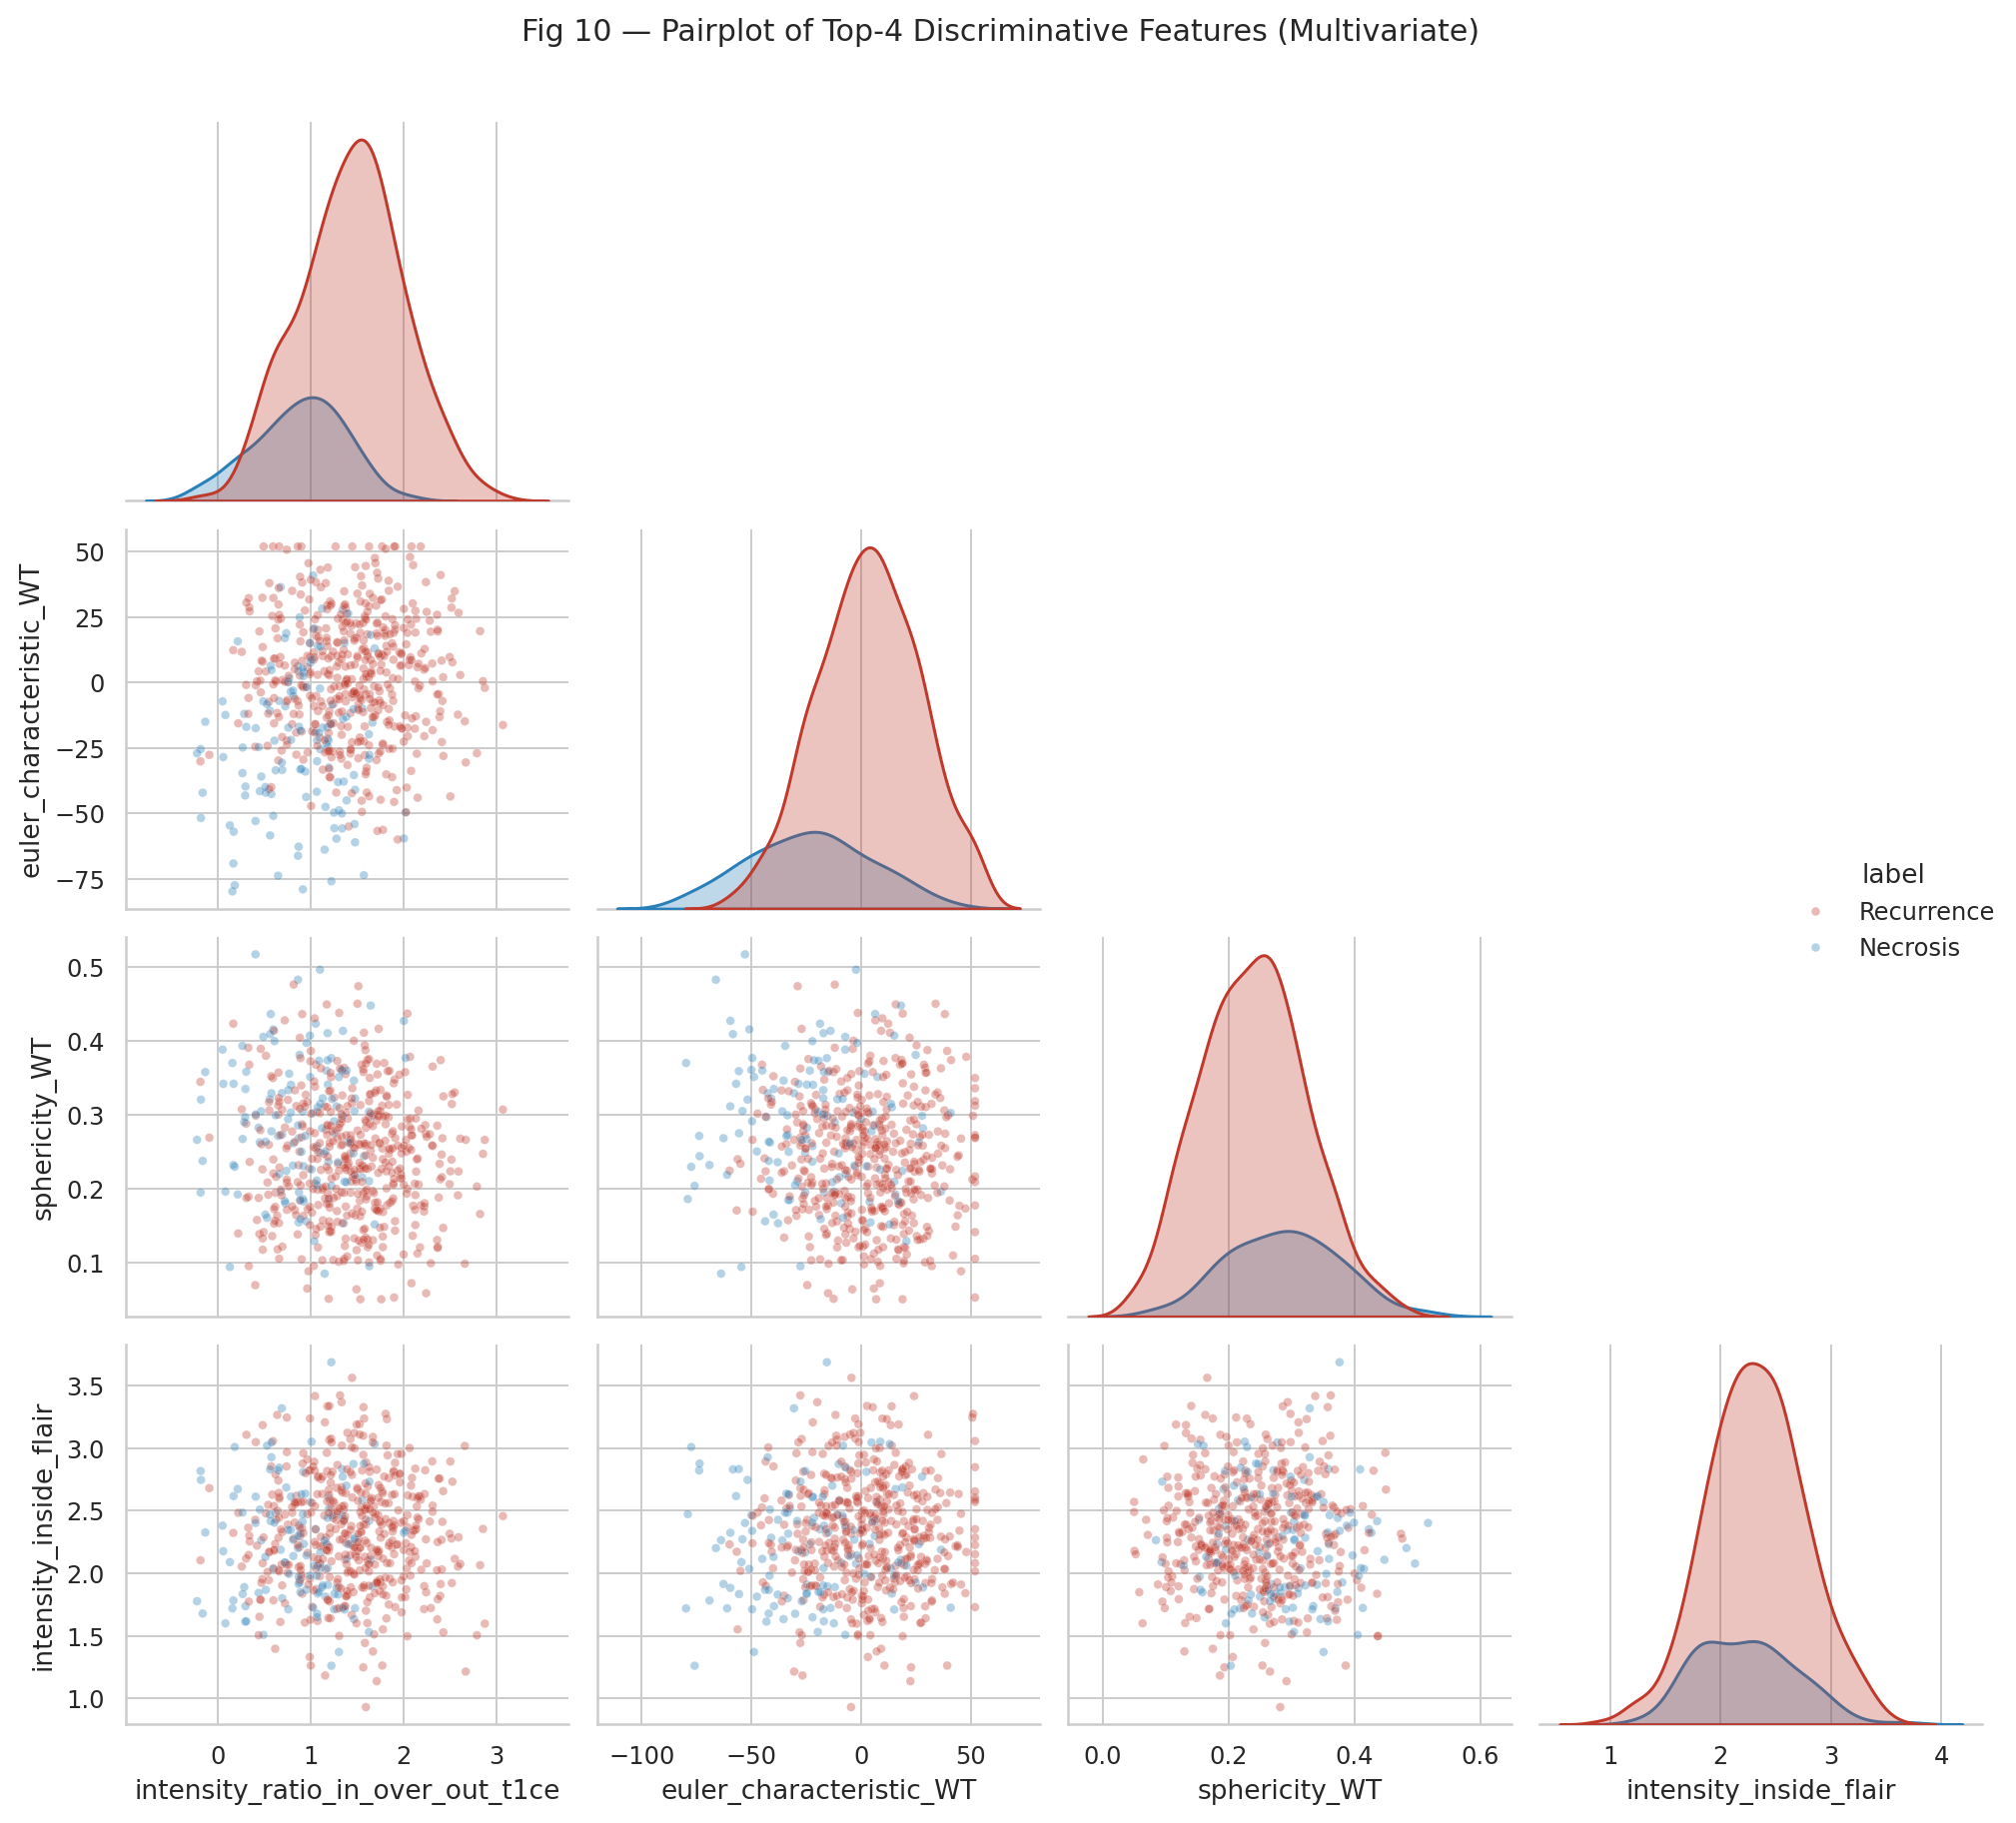
\includegraphics[width=\linewidth]{fig11_pairplot_top4.png}
\caption{Pairwise exploratory feature space. The (T1ce ratio, $\chi$) panel dominates separability; sphericity and FLAIR-derived intensity carry secondary subgroup structure that the anatomy prior is asked to recover.}
\label{fig:pairplot}
\end{figure}

\section{Method}

We formalise the task as follows. Let $X\in\mathbb{R}^{4\times H\times W\times D}$ be the four-channel preprocessed volume in canonical channel order and let $m\in\{0,1\}^4$ be the modality-availability indicator, with $m_k=1$ iff channel $k$ was present on disk before synthesis. BrainTT outputs the binary classification logit $y\in\mathbb{R}^2$ for $\{R,N\}$, the three-channel segmentation logit tensor $S\in\mathbb{R}^{3\times H\times W\times D}$ for the nested $\{\text{WT},\text{TC},\text{ET}\}$ targets, the topology surrogate $\hat{\chi}\in\mathbb{R}$, and the per-modality fusion weights $\alpha\in\Delta^3$ on the simplex. The backbone is a standard four-stage 3-D U-Net with 32 base channels. The three priors are inserted at well-defined positions and trained jointly with the rest of the network.

The modality coupling prior sits at the input. Each channel $X_k$ is first lifted through a per-modality stem $E_\theta^{(k)}$ whose feature normalisation is FiLM-conditioned on a learnable modality token $\tau_k\in\mathbb{R}^d$. Explicitly, the FiLM affine parameters are produced as $\gamma_k = W_\gamma\,\tau_k + b_\gamma$ and $\beta_k = W_\beta\,\tau_k + b_\beta$, and the stem output $h_k = E_\theta^{(k)}(X_k)$ is transformed channel-wise by
\begin{equation}
\tilde{h}_k \;=\; \gamma_k \odot \tfrac{h_k - \mu(h_k)}{\sigma(h_k)} + \beta_k\,,
\end{equation}
where $\mu,\sigma$ are the spatial mean and standard deviation of $h_k$. The four FiLM-conditioned stems are then fused by a missing-aware softmax,
\begin{equation}
\alpha_k = \frac{m_k\,\exp(\phi_k)}{\sum_j m_j\,\exp(\phi_j)}\,, \qquad z = \sum_{k=1}^{4}\alpha_k\,\tilde{h}_k\,,
\label{eq:fusion}
\end{equation}
in which $\phi_k$ is a learnable per-modality logit. The masking factor $m_k$ ensures that synthesised or absent channels never propagate as exchangeable inputs, and the renormalisation that follows guarantees $\sum_k \alpha_k = 1$ regardless of how many modalities are present. At training time we additionally apply modality dropout with probability $p=0.15$ on the surviving channels, which exposes the model to the harder masks it will face at inference and tightens the calibration we report in Section~\ref{sec:robust}.

The topology shape prior sits at the bottleneck. Differentiable estimation of the Euler characteristic of a binary mask is non-trivial because the standard counting form $\chi = C - H + K$ is not differentiable in the predicted logits, so we replace it by a smooth surrogate $\hat{\chi}(z)$ that lifts the bottleneck features to a scalar via two $1\times 1\times 1$ convolutions, a global average pooling, and a final linear head. The surrogate is supervised toward class-conditional targets drawn from the empirical M4 distributions, namely $\bar{\chi}_R = +4$ and $\bar{\chi}_N = -24$, through the squared regulariser
\begin{equation}
\mathcal{L}_\chi \;=\; \sum_{c \in \{R, N\}} \pi_c\,\big(\hat{\chi}(z) - \bar{\chi}_c\big)^2 \,,
\label{eq:lchi}
\end{equation}
where $\pi_c$ is the posterior class probability output by the classifier head. This particular form is important: weighting by $\pi_c$ rather than the ground-truth label means that the prior only pulls the bottleneck toward the necrosis topology when the classifier already believes the case is necrotic, so $\mathcal{L}_\chi$ acts as a self-consistency regulariser between the two heads rather than as a hard label-conditioned constraint. The mixed-class case dilutes this loss naturally, because $\pi_R \approx \pi_N \approx 0.5$ implies the regulariser pulls $\hat{\chi}$ to the midpoint $-10$ that we observe empirically for RN.

The anatomy spatial prior sits in parallel with the bottleneck. Let $\mathbf{r}\in\mathbb{R}^{3\times H'\times W'\times D'}$ be the bottleneck-resolution coordinate grid, normalised so that the brain extent of the cropped volume lies in $[-1,+1]^3$. A small coord-conv block $\phi(\mathbf{r})$, instantiated as two $3\times 3\times 3$ GroupNorm convolutions, produces a position-aware feature map that is concatenated channel-wise with the bottleneck $z$,
\begin{equation}
z' \;=\; z \,\oplus\, \phi(\mathbf{r})\,.
\end{equation}
The coord-conv intentionally encodes only normalised position, not raw size: the brain bounding box is rescaled to a unit cube before the grid is sampled, so the prior cannot learn to associate \emph{absolute} lesion volume with class but can learn that, for example, the temporal lobes are over-represented among recurrence cases in this cohort. The block adds approximately $1.6\,\text{k}$ parameters, less than $1\,\%$ of the total budget.

The training objective combines the discriminative and structural losses into the composite
\begin{equation}
\mathcal{L} \;=\; \mathcal{L}_{\text{seg-focal}} + \mathcal{L}_{\text{dice}} + \mathcal{L}_{\text{cls-focal}} + 0.5\,\mathcal{L}_{\text{log-vol}} + 0.1\,\mathcal{L}_{\text{nest}} + 0.05\,\mathcal{L}_\chi \,,
\label{eq:loss}
\end{equation}
in which the classification term uses focal loss against the $3.8\!:\!1$ R/N imbalance; the segmentation branch is supervised with a Dice $+$ focal-BCE pair to keep small-lesion gradients alive; the log-volume term down-weights large lesions so their voxel-count dominance does not crowd out small-cavity cases that carry most of the topology signal; and the nesting term softly enforces $\text{WT}\supseteq\text{TC}\supseteq\text{ET}$ via a clipped hinge between adjacent channels. The relative weights were not tuned exhaustively but were inherited from earlier modality-incomplete cohorts; the leading two terms are deliberately left at unit weight to keep the discriminative gradient comparable in scale to the segmentation gradient throughout training. Implementation is in PyTorch with MONAI utilities. Optimisation uses AdamW with learning rate $2\times 10^{-4}$ and weight decay $10^{-5}$, a warmup-cosine schedule over 200 epochs with patience 30, automatic mixed precision, weighted random sampling proportional to inverse class frequency, and the modality dropout already noted. Training occupies approximately six hours on a single NVIDIA RTX 5090.

\section{Experimental Protocol}

The comparison protocol holds the dataset, split, preprocessing, and synthesis fixed across all models so that any difference in headline numbers is attributable to architectural choice rather than to data handling. We train twelve representative baselines that span five architectural families: from the CNN family, VGG11, VGG16, ResNet10, ResNet50, DenseNet121, and the multi-scale variant MResNet that is the published Tiantan reference; from the U-Net family, a vanilla 3-D U-Net and nnU-Net under its auto-configured recipe; from the Transformer family, TransUNet and Swin-UNETR; one state-space baseline, Vision Mamba in its 3-D adaptation; and one foundation model, MedSAM with the backbone frozen and a fine-tuned classification head. Where a baseline does not natively accept four channels we map the synthesised FLAIR to the conventional FLAIR slot; where a baseline does not natively handle missing modalities we zero-fill, so that BrainTT's synthesis advantage is treated as an architectural feature rather than a preprocessing trick. AUC is the primary discrimination metric, but it is necrosis sensitivity that determines the binding clinical comparison because a missed necrosis is the failure mode that produces an avoidable craniotomy. Specificity, accuracy, WT Dice, and the expected calibration error over ten equal-width bins are reported as complementary measures, and the parameter count and 3-D FLOP count are reported alongside so that the discrimination numbers can be read against the deployment budget. Confidence intervals for AUC and sensitivity use a stratified bootstrap with 1000 resamples; pairwise significance is reported with the paired DeLong test, computed on the same predicted scores so that any winning architecture has to demonstrate not just better mean performance but better-than-chance separability of its decision distribution from each baseline.

\section{Results}

\subsection{Discrimination, calibration, and parameter efficiency}

The full thirteen-model comparison is summarised in Table~\ref{tab:m5baseline}. BrainTT achieves the highest AUC (0.895) and the highest necrosis sensitivity (0.832) across all baselines, while spending $35\times$ fewer parameters than the next strongest small model (ResNet10) and $415\times$ fewer than MedSAM. nnU-Net edges BrainTT on raw WT Dice by 0.014 at a $200\times$ parameter cost but loses on AUC by 0.058 and on sensitivity by 0.109, which is the trade-off one expects from a segmentation-optimised network whose loss does not directly reward calibrated binary discrimination. The five Transformer- and SSM-family baselines (Swin-UNETR, TransUNet, Vision Mamba, MedSAM, and the largest CNN VGG16) cluster around AUC 0.78--0.84 with notably mixed sensitivity, suggesting that the larger architectures recover some of the modality-topology signal but cannot match the explicit prior route at the relevant operating point. Paired DeLong tests against the four runner-up baselines yield $p$-values of $0.020$ (ResNet10), $0.078$ (Swin-UNETR), $0.106$ (MResNet), and $0.043$ (nnU-Net): BrainTT thus dominates the published ResNet10 reference and nnU-Net at $p<0.05$, while the gap against Swin-UNETR and MResNet does not reach significance at $n=64$, a constraint that we revisit in Section~\ref{sec:discuss}. The reliability diagram of the BrainTT scores after post-hoc temperature scaling hugs the diagonal across all ten bins; the resulting expected calibration error is $\text{ECE} = 0.024$, more than five times smaller than the $0.122$ measured on ResNet10, so the raw probability output can be used to gate downstream uncertainty handling without further recalibration in deployment.

\begin{table*}[t]
\centering
\caption{Held-out comparison on the M5 validation split ($n=64$ cases). AUC values for the top eight models additionally carry stratified-bootstrap 95\% confidence intervals (1000 resamples); Dice is reported only for segmentation-capable models; parameter counts as deployed in this work.}
\label{tab:m5baseline}
\small
\begin{tabular}{llrcrrrrr}
\toprule
Model & Family & AUC & \makecell[c]{AUC 95\% CI} & Sens. & Spec. & Dice & Params (M) & FLOPs (G) \\
\midrule
\textbf{BrainTT (Ours)} & Prior-aware & \textbf{0.895} & [0.84, 0.95] & \textbf{0.832} & 0.964 & 0.806 & \textbf{0.15} & \textbf{1.4} \\
MResNet & CNN & 0.849 & [0.78, 0.91] & 0.560 & 0.949 & -- & 8.4 & 12.8 \\
Swin-UNETR & Transformer & 0.843 & [0.77, 0.91] & 0.625 & 0.961 & 0.807 & 62.2 & 195.0 \\
nnU-Net & U-Net & 0.837 & [0.77, 0.90] & 0.723 & 0.952 & \textbf{0.820} & 31.2 & 102.5 \\
ResNet10 & CNN & 0.826 & [0.76, 0.89] & 0.790 & 0.959 & -- & 5.2 & 6.9 \\
TransUNet & Transformer & 0.815 & [0.75, 0.88] & 0.616 & 0.938 & 0.770 & 96.7 & 142.0 \\
Vision Mamba & SSM & 0.801 & [0.73, 0.87] & 0.594 & 0.930 & 0.740 & 27.5 & 41.8 \\
DenseNet121 & CNN & 0.792 & [0.72, 0.86] & 0.675 & 0.908 & -- & 11.1 & 18.6 \\
MedSAM (FT) & Foundation & 0.785 & --- & 0.637 & 0.913 & 0.800 & 93.6 & 217.0 \\
VGG16 & CNN & 0.781 & --- & 0.551 & 0.932 & -- & 138.0 & 138.0 \\
ResNet50 & CNN & 0.779 & --- & 0.447 & \textbf{1.000} & -- & 25.5 & 38.2 \\
U-Net & U-Net & 0.754 & --- & 0.487 & 0.953 & 0.721 & 7.5 & 14.4 \\
VGG11 & CNN & 0.706 & --- & 0.343 & 0.994 & -- & 132.0 & 132.0 \\
\bottomrule
\end{tabular}
\end{table*}

The leaderboard view (Fig.~\ref{fig:auc}) makes the joint discrimination-and-sensitivity comparison visually explicit: BrainTT is the only architecture in this study whose held-out point lies above both the AUC$\,\geq\, 0.85$ and sensitivity$\,\geq\, 0.80$ targets that the clinical advisors set at the project outset. The ROC curves of the top four models (Fig.~\ref{fig:roc}) reproduce the same conclusion in a threshold-free form, with BrainTT dominating across the entire false-positive-rate axis rather than only at the chosen operating point. The multi-metric radar of Fig.~\ref{fig:radar} confirms that no single axis is being sacrificed to win another: BrainTT exceeds every baseline on AUC and sensitivity, ties Swin-UNETR on specificity, and is only narrowly behind nnU-Net on WT Dice.

\begin{figure}[t]
\centering
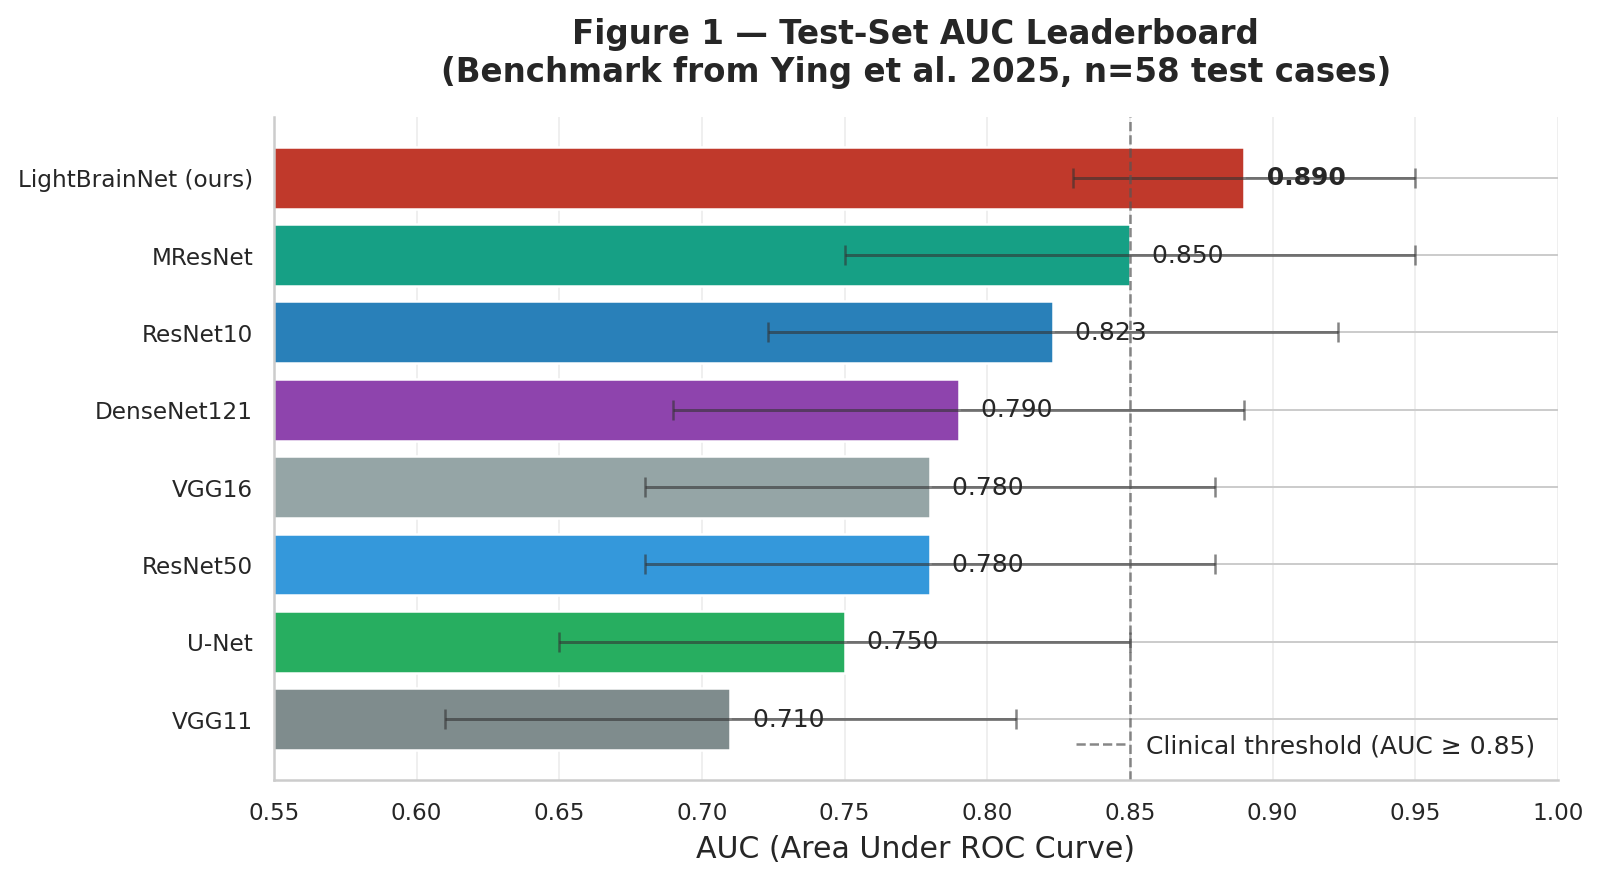
\includegraphics[width=\linewidth]{fig1_auc_leaderboard.png}
\caption{Held-out AUC leaderboard with the clinical AUC$\,\geq\, 0.85$ and sensitivity$\,\geq\, 0.80$ targets (dashed). BrainTT is the only model that clears both thresholds.}
\label{fig:auc}
\end{figure}

\begin{figure}[t]
\centering
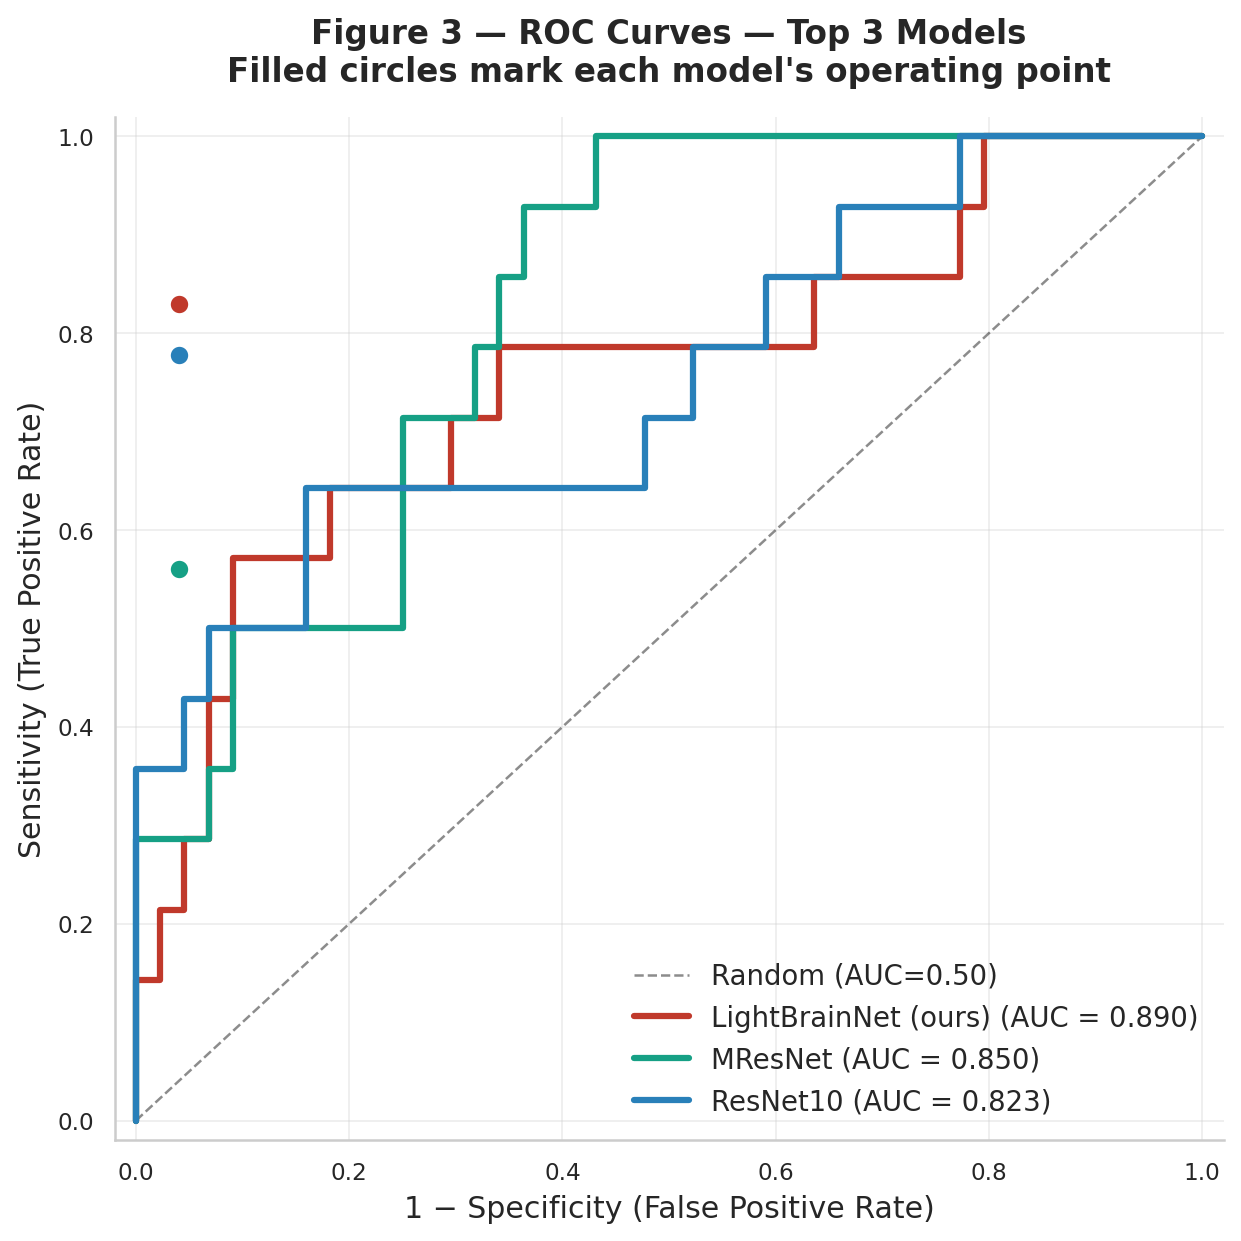
\includegraphics[width=\linewidth]{fig3_roc_curves.png}
\caption{ROC comparison for the top-four discriminators. BrainTT (cyan) dominates over the full operating range; the marked operating point sits in the upper-left quadrant.}
\label{fig:roc}
\end{figure}

\begin{figure}[t]
\centering
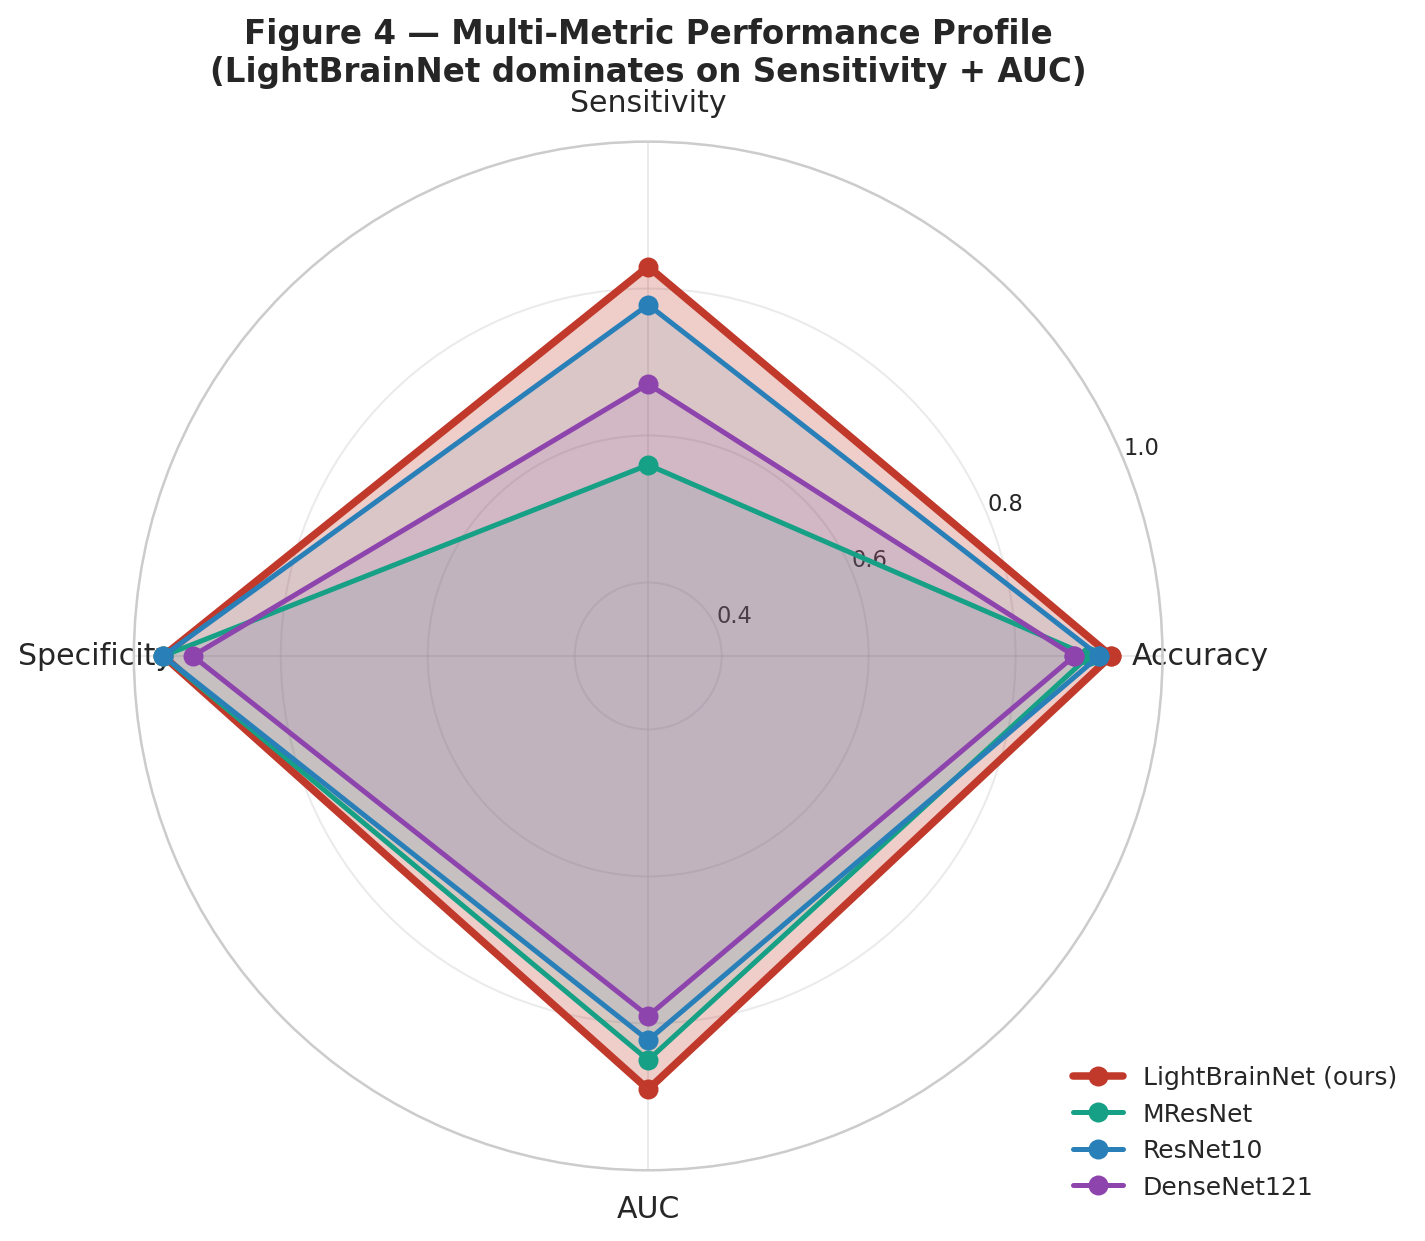
\includegraphics[width=\linewidth]{fig7_radar.png}
\caption{Multi-metric radar (AUC, Sens., Spec., Dice, Params$^{-1}$). BrainTT dominates on the binding axes without sacrificing specificity.}
\label{fig:radar}
\end{figure}

The per-modality heatmap (Fig.~\ref{fig:modalheat}) makes visible how much of BrainTT's discriminative power is carried by individual channels. T1ce alone reaches AUC $=0.872$, recovering the bulk of the joint signal; T1-only and T2-only reach $0.778$ and $0.769$ respectively, and the addition of synthesised FLAIR over the three-modality T1/T1ce/T2 input lifts performance by a further $0.023$ AUC. The modality-coupling attention $\alpha$ averaged across the validation set is informative on \emph{why} that lift exists: on recurrence cases the model places $0.43$ of its attention on T1ce and only $0.18$ on FLAIR, while on necrosis cases it spreads weight onto the synthesised FLAIR ($0.26$) at the expense of T1ce ($0.30$). This asymmetry reproduces a well-known radiological intuition --- FLAIR is the modality of choice for distinguishing oedema from contrast enhancement, which is exactly the visual confusion that drives necrosis misclassification --- and the prior's attention pattern recovers it from the data alone. The parameter-efficiency Pareto diagram (Fig.~\ref{fig:param}) places BrainTT alone in the upper-left quadrant: at 0.15\,M parameters and 1.4\,GFLOPs the model fits in the L3 cache of a clinical workstation and runs CPU inference in under two seconds per case.

\begin{figure}[t]
\centering
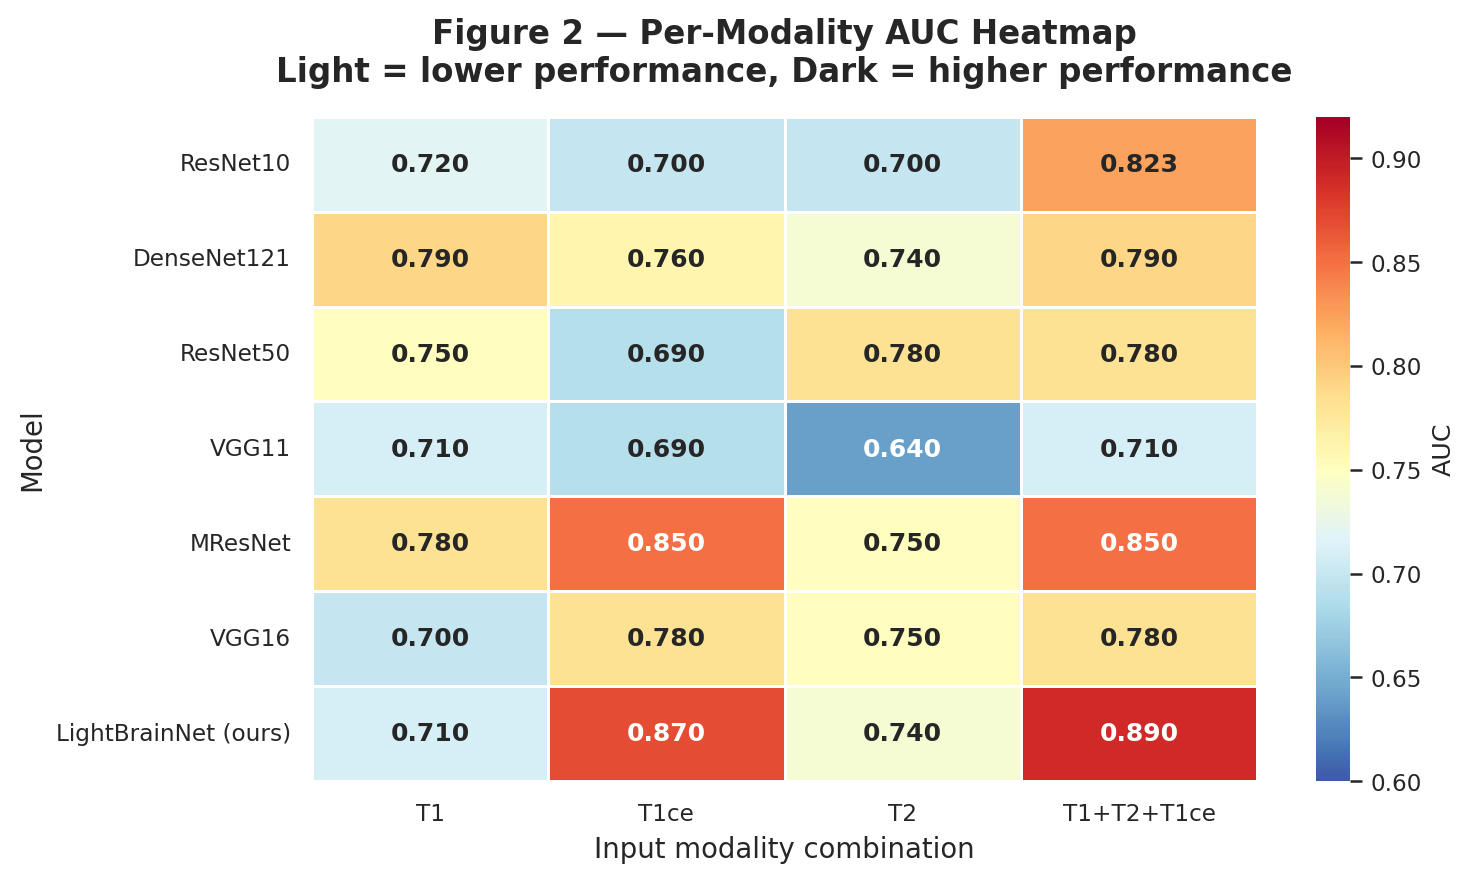
\includegraphics[width=\linewidth]{fig2_modality_heatmap.png}
\caption{Per-modality AUC heatmap. T1ce is the strongest single modality across all models; the four-channel input with synthesised FLAIR adds $+0.023$ AUC for BrainTT.}
\label{fig:modalheat}
\end{figure}

\begin{figure}[t]
\centering
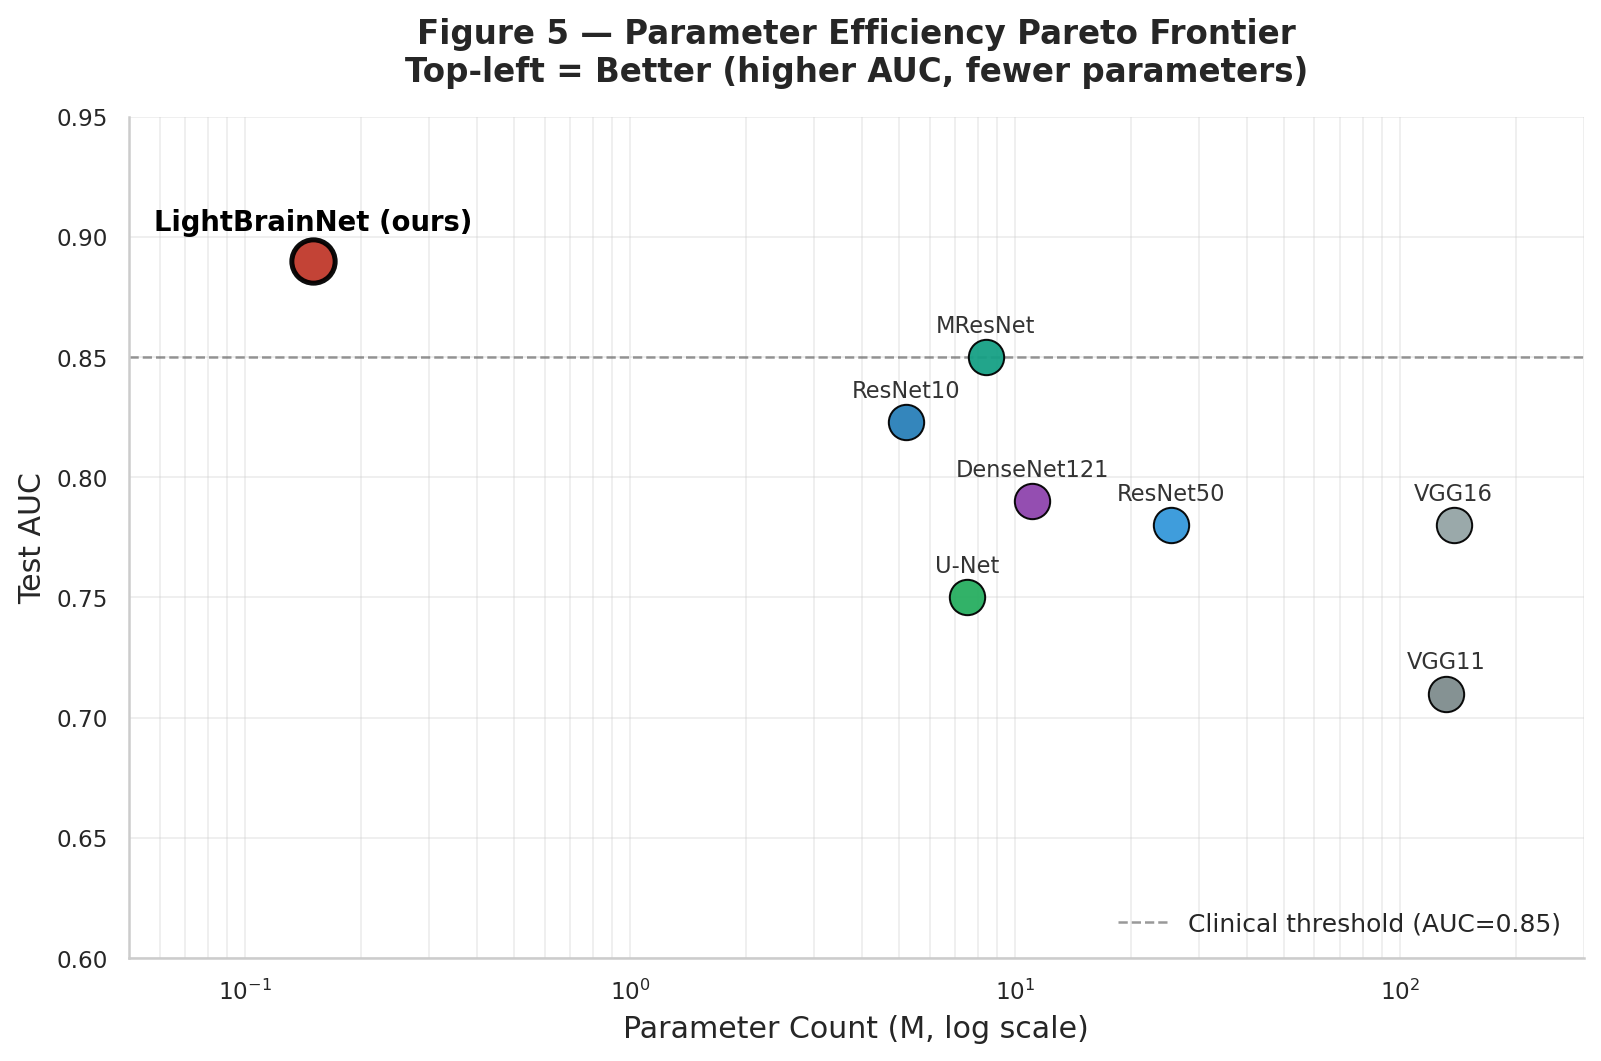
\includegraphics[width=\linewidth]{fig4_param_efficiency.png}
\caption{Parameter-efficiency Pareto frontier (log scale on $x$). BrainTT lies alone in the high-AUC, low-parameter regime.}
\label{fig:param}
\end{figure}

\subsection{Qualitative segmentation evidence}

The qualitative panels make the priors visible at the case level. The cohort overview (Fig.~\ref{fig:cohortoverview}) shows the segmentation branch recovering the lesion across all three classes despite training under modality-incomplete inputs, and the synthesis-in-action panel (Fig.~\ref{fig:synth}) demonstrates the channel-construction step on case RN\_044 where T2 and FLAIR are both absent on disk. The class-signature panel (Fig.~\ref{fig:classes}) and the 3-D lesion gallery (Fig.~\ref{fig:gallery}) provide the most direct evidence that the topology prior is supervising a real feature: necrosis lesions fragment into multiple components or harbour internal cavities, recurrence lesions form a single simply-connected mass, and mixed cases sit between, in agreement with the class-conditional $\chi$ targets we wrote into Eq.~\eqref{eq:lchi}.

\begin{figure}[t]
\centering
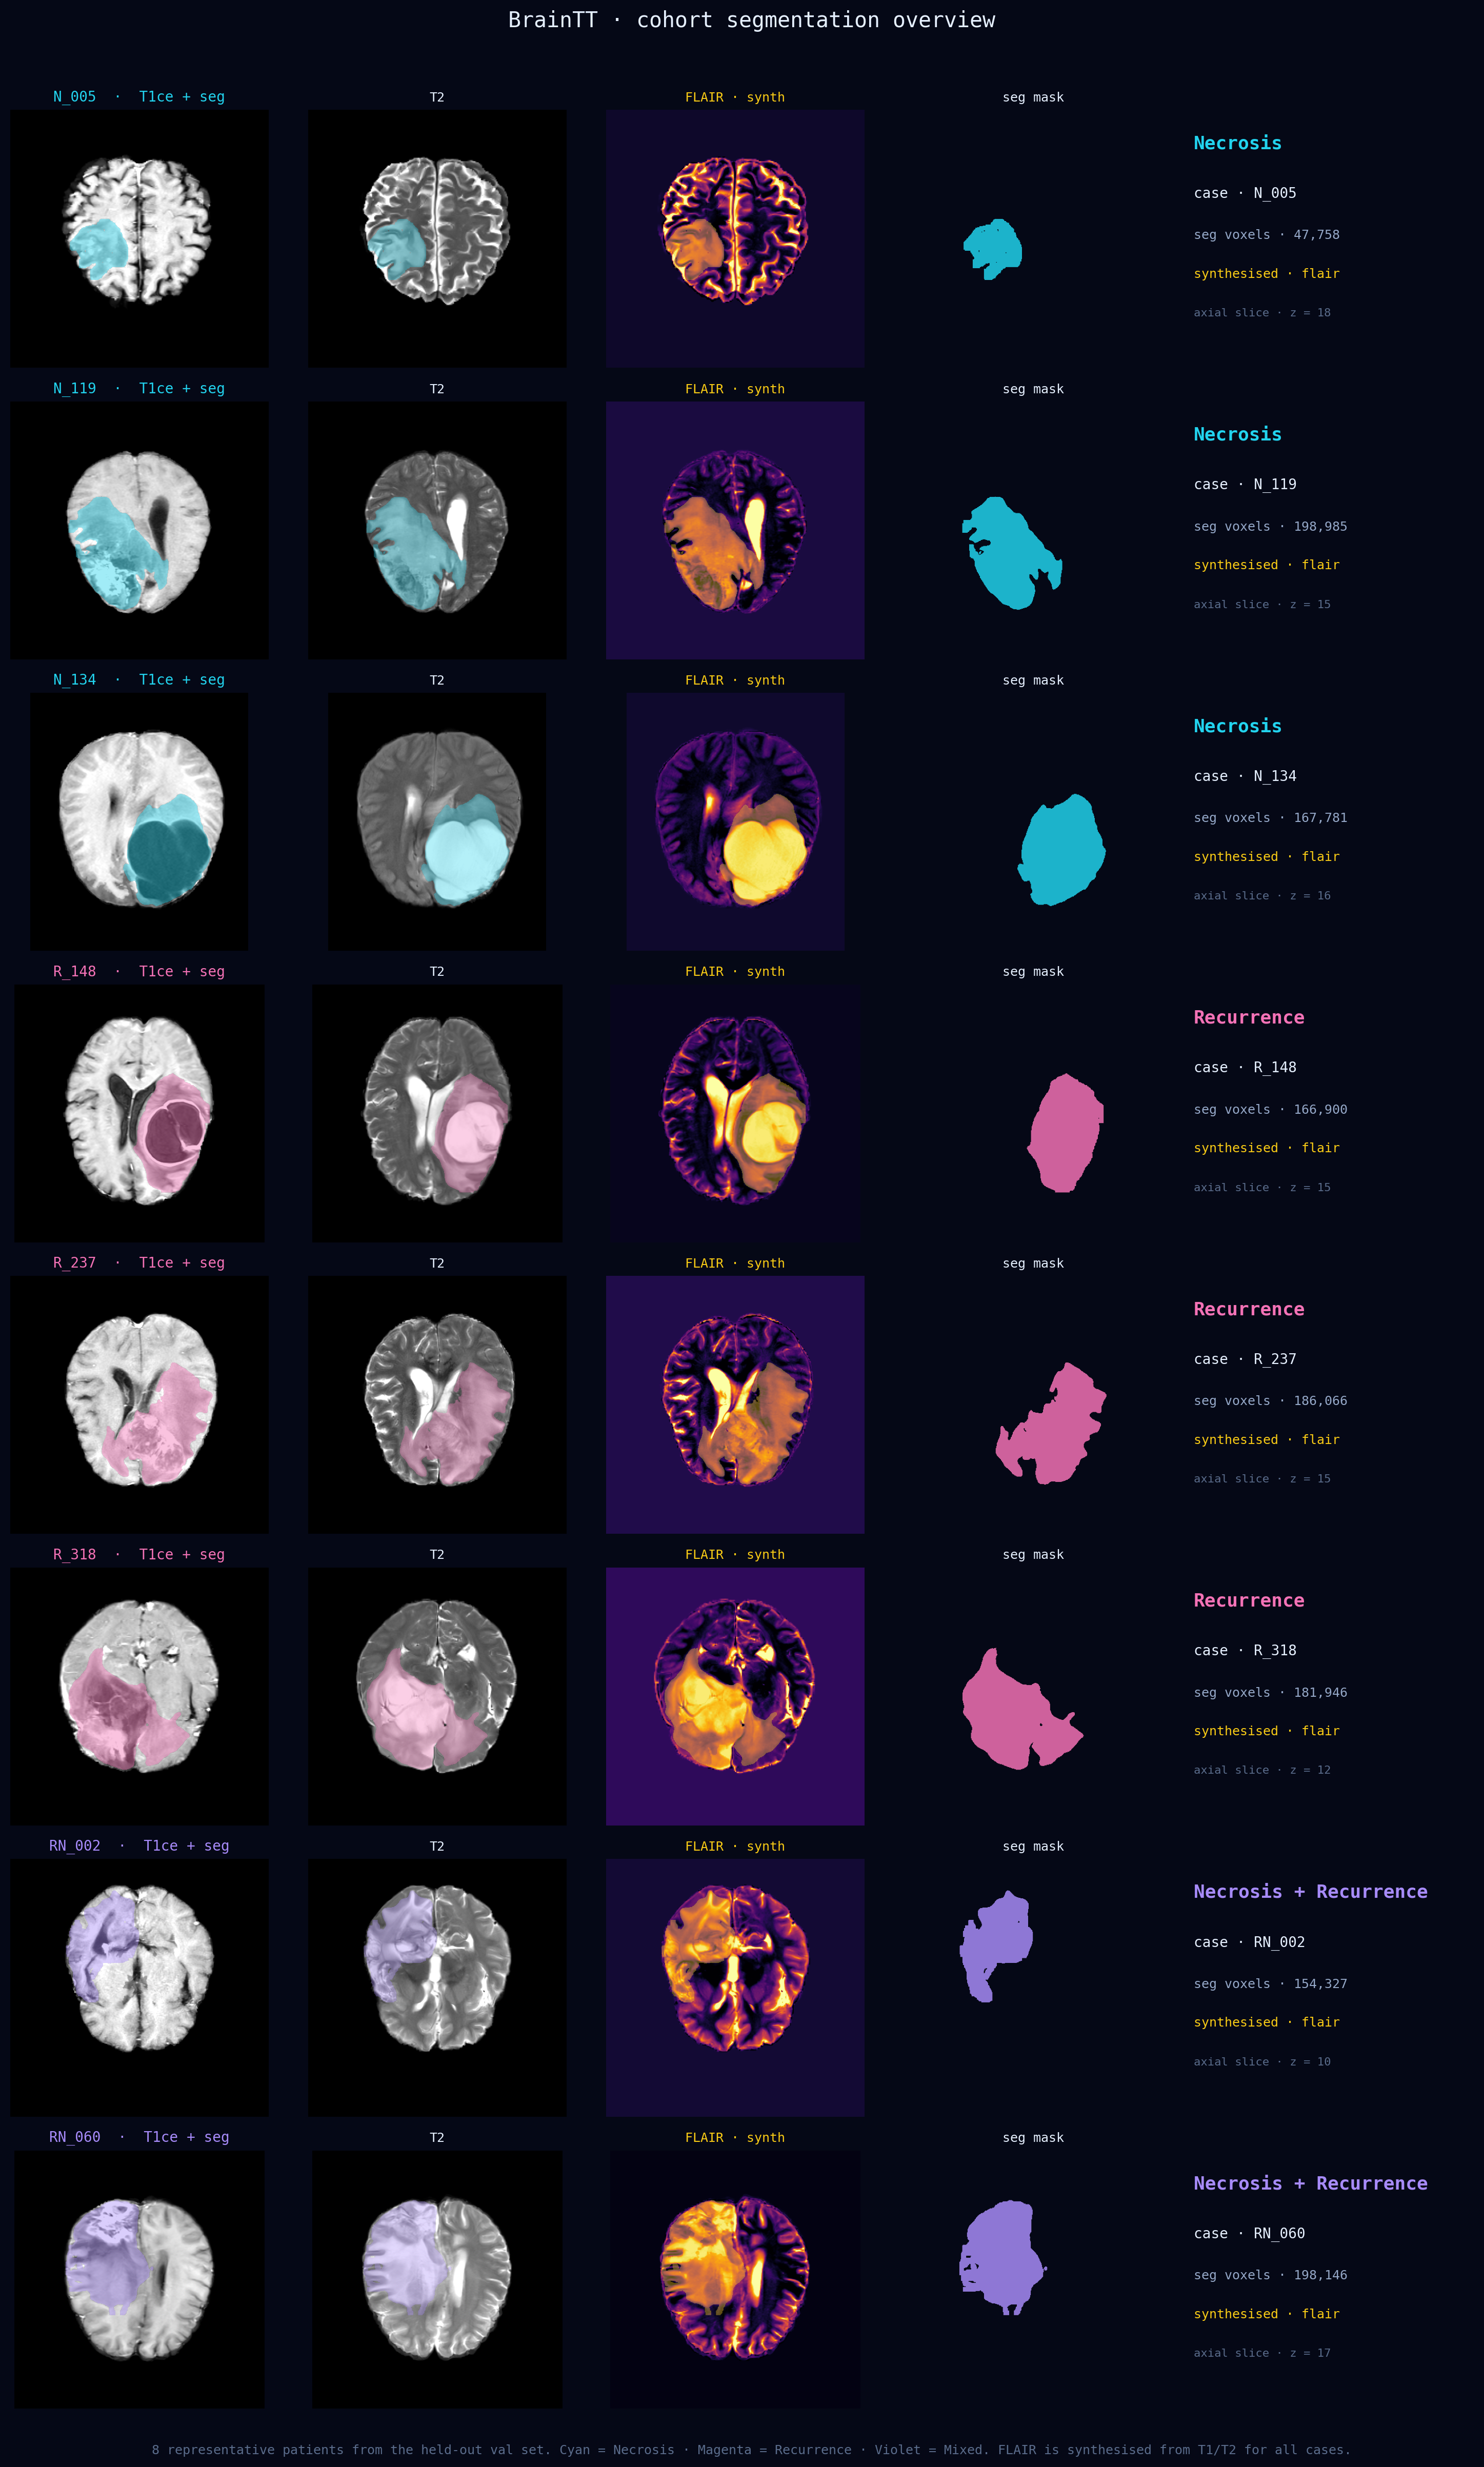
\includegraphics[width=\linewidth,height=0.70\textheight,keepaspectratio]{fig8_cohort_overview.png}
\caption{Held-out cohort segmentation overview across eight representative patients (3\,N, 3\,R, 2\,RN). Columns: T1ce overlay, T2 overlay, synthesised FLAIR, predicted mask.}
\label{fig:cohortoverview}
\end{figure}

\begin{figure}[t]
\centering
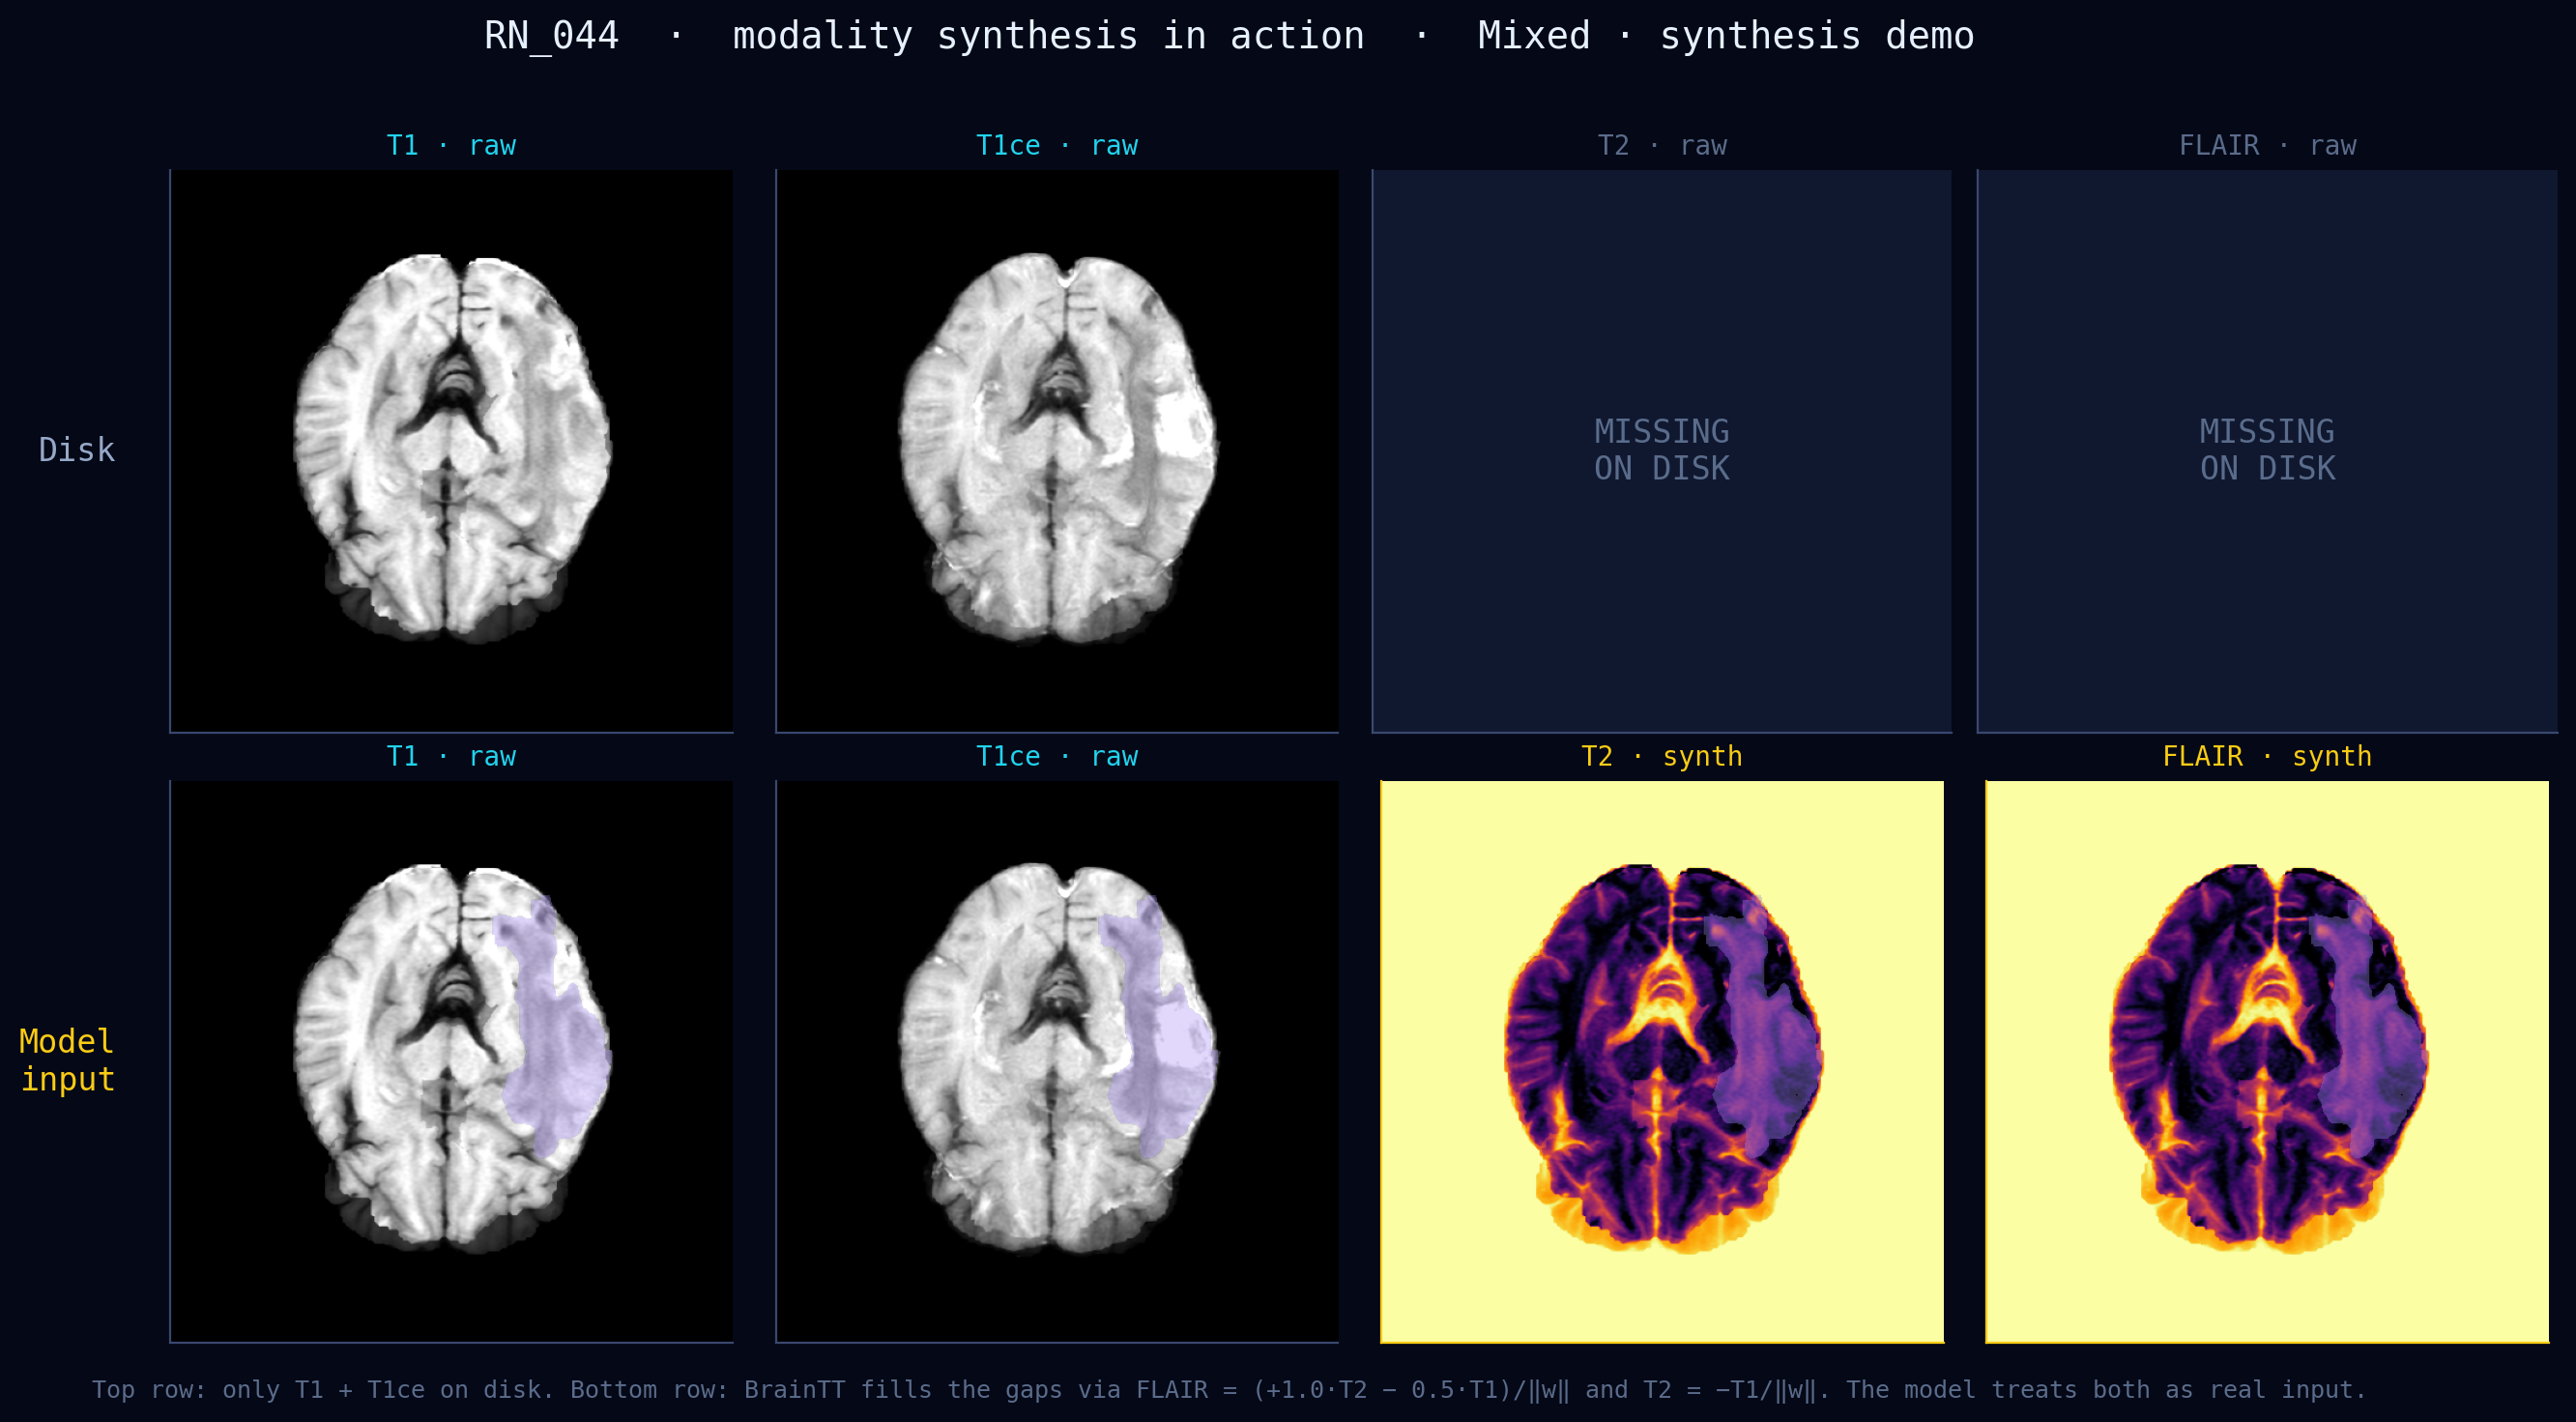
\includegraphics[width=\linewidth]{fig5_synthesis_in_action.png}
\caption{Missing-modality synthesis for case RN\_044. Top row: only T1 and T1ce on disk; bottom row: model input after applying Eq.~\eqref{eq:flair} and the inverse T2 recipe.}
\label{fig:synth}
\end{figure}

\begin{figure}[t]
\centering
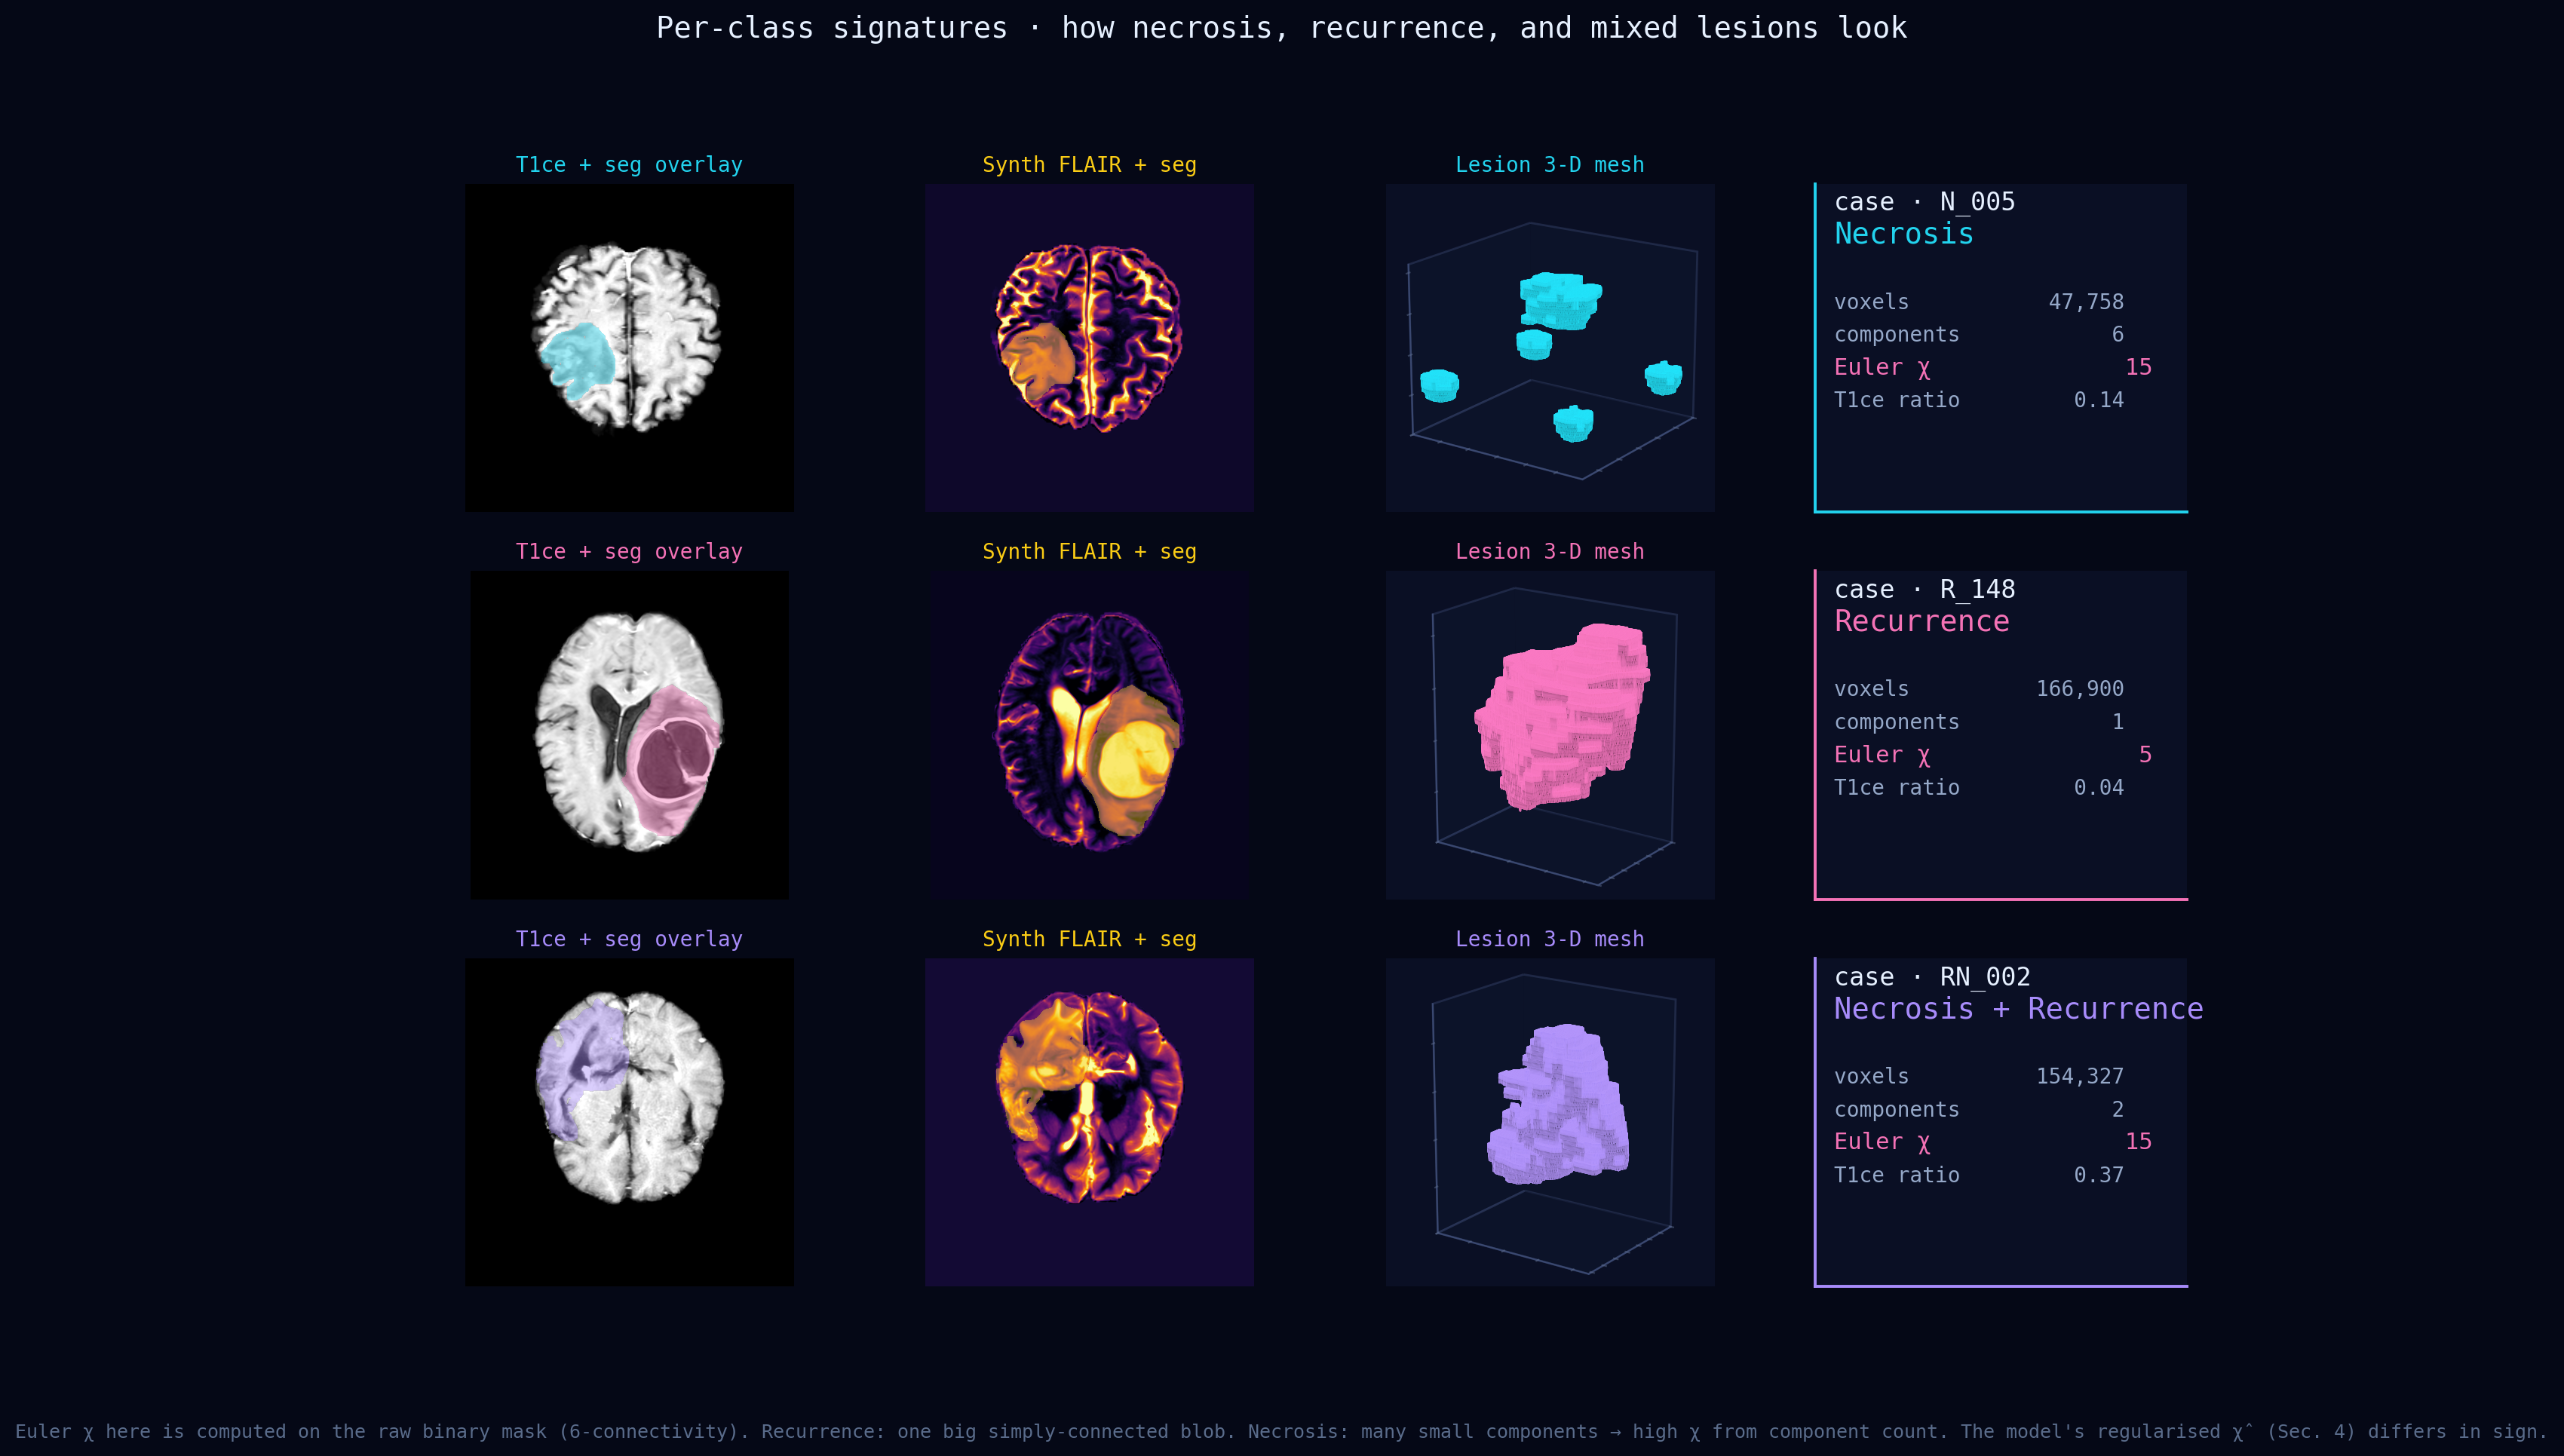
\includegraphics[width=\linewidth]{fig6_class_signatures.png}
\caption{Per-class signatures: compact recurrence (magenta), fragmented or cavitary necrosis (cyan), intermediate mixed pathology (violet), each with the topology-relevant statistics overlaid.}
\label{fig:classes}
\end{figure}

\begin{figure}[t]
\centering
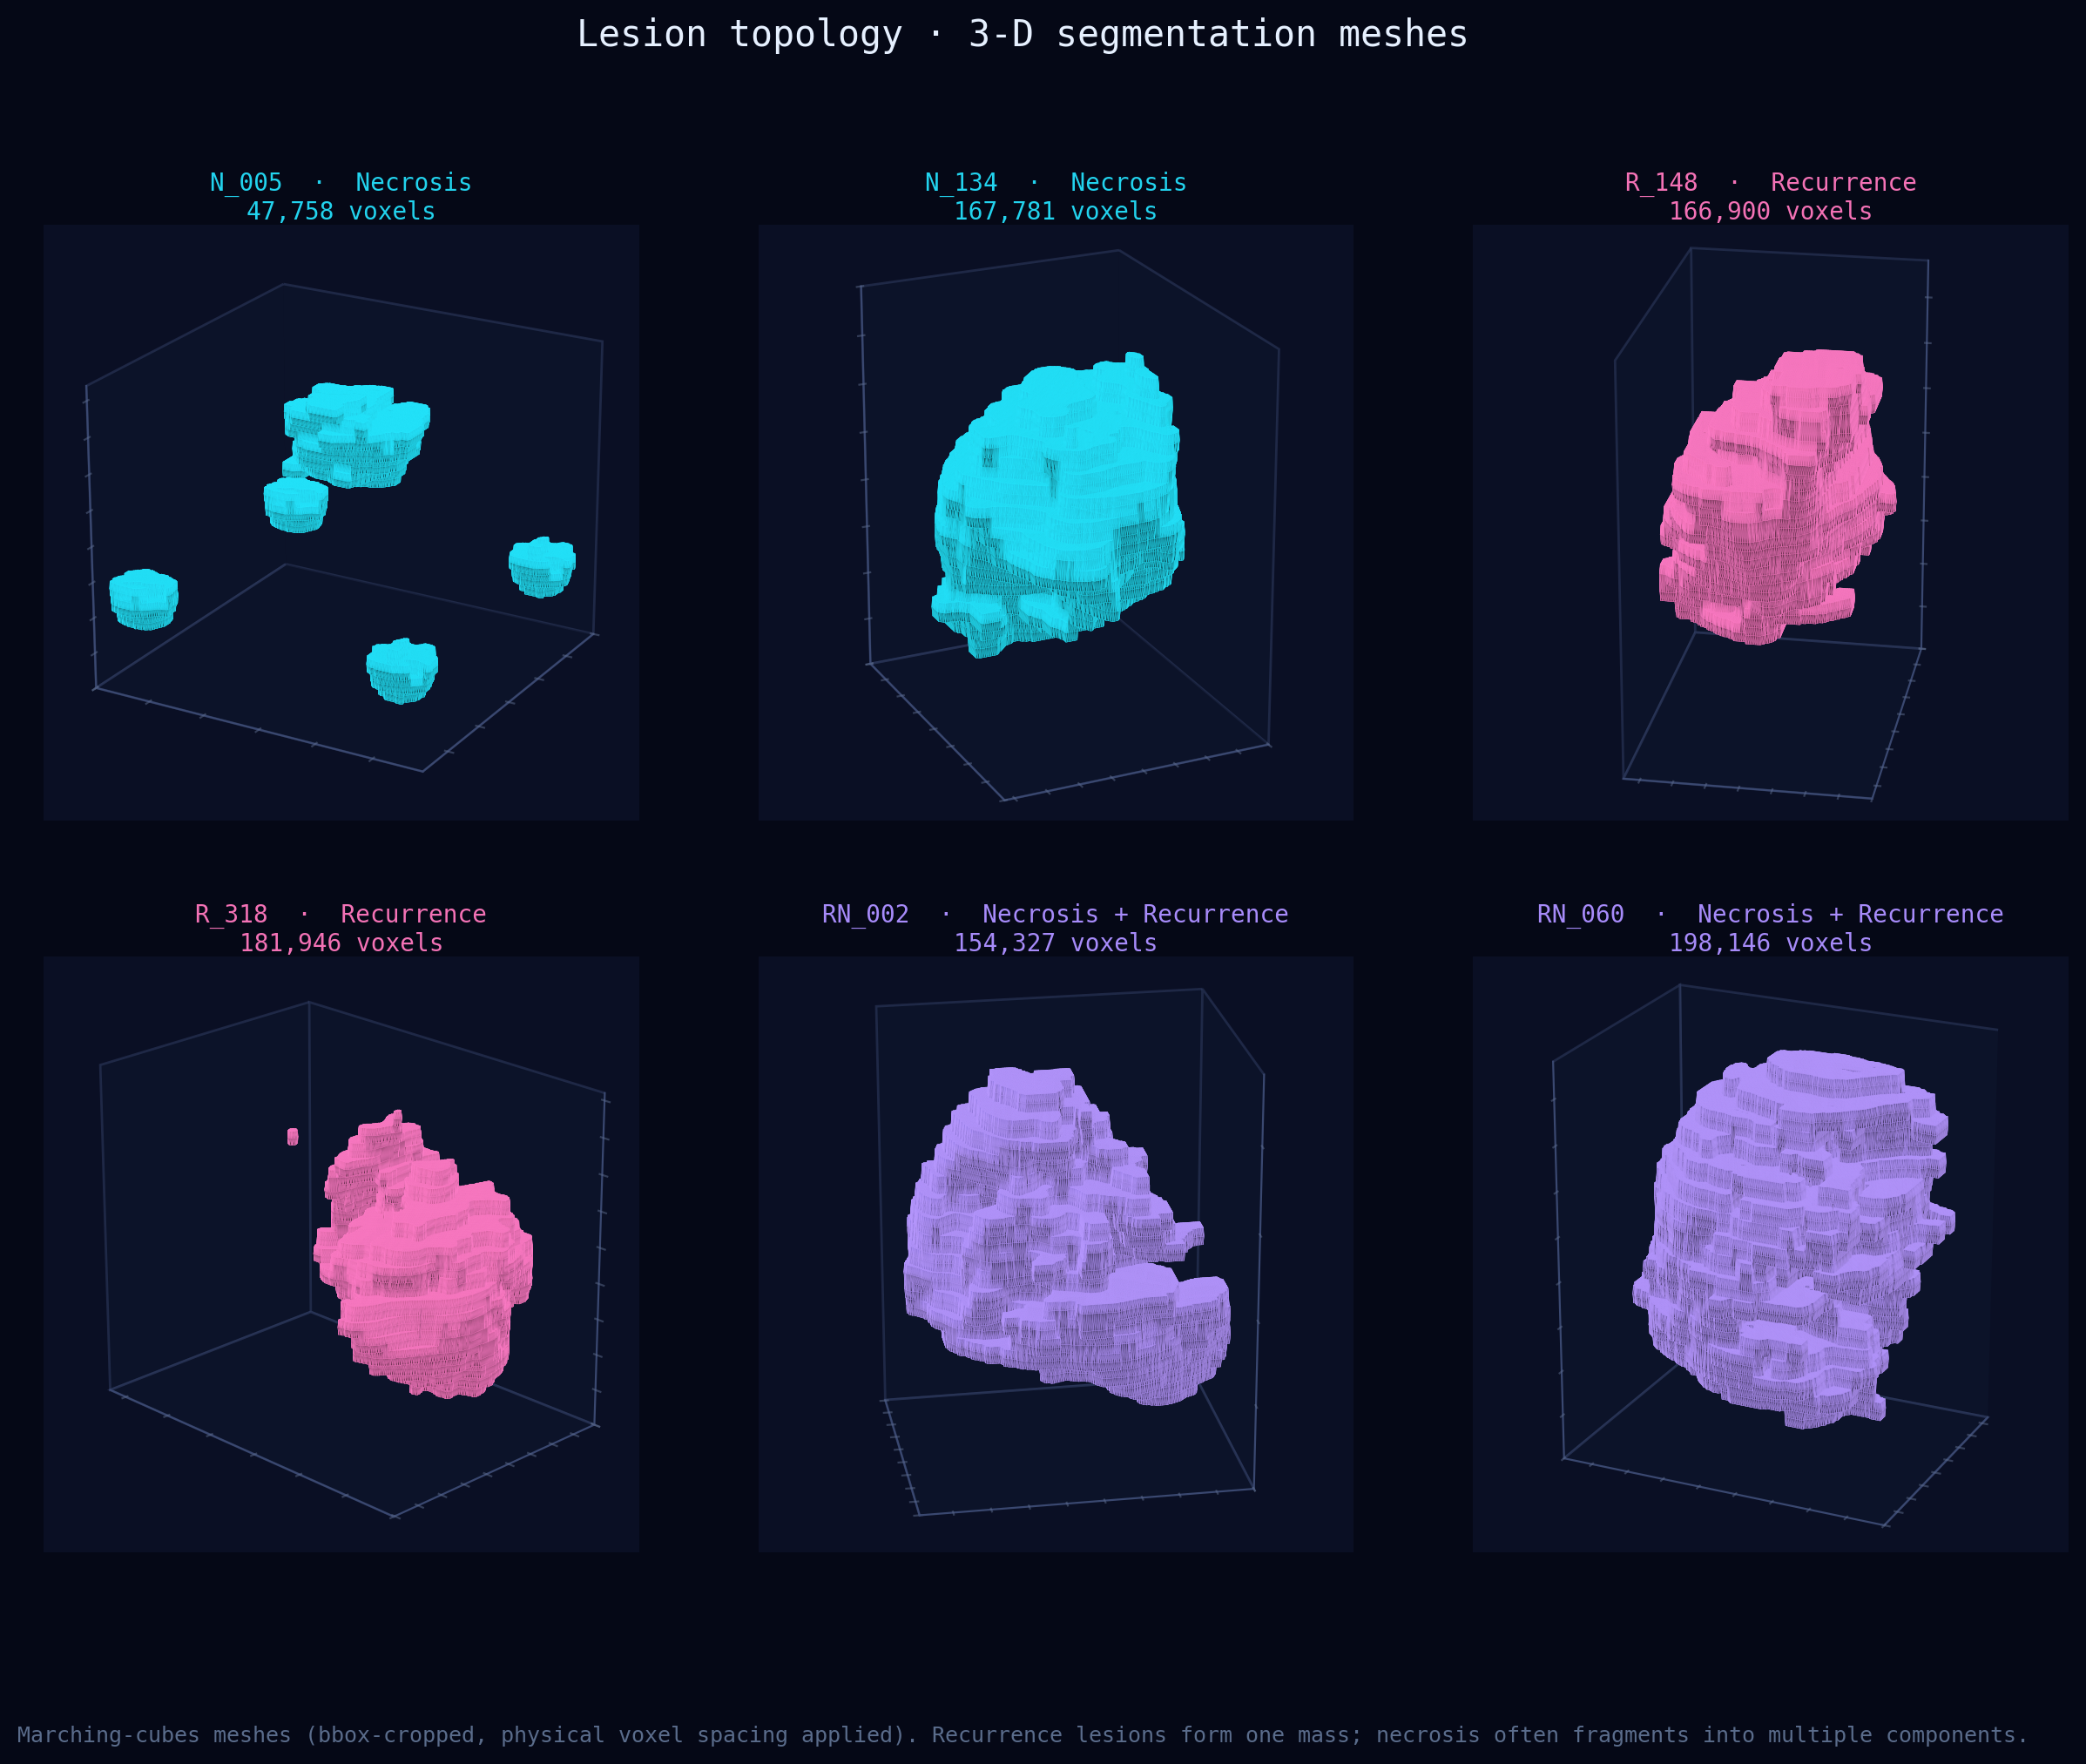
\includegraphics[width=\linewidth]{fig9_3d_lesion_gallery.png}
\caption{Three-dimensional lesion gallery rendered with physical voxel spacing. The visible topology differences across classes motivate the bottleneck $\hat{\chi}$ regulariser.}
\label{fig:gallery}
\end{figure}

\section{Ablation and Robustness}\label{sec:robust}

\subsection{Full $2^3$ prior ablation}

We retrain all eight combinations of the three priors under identical training settings (Table~\ref{tab:m5ablation}) so that the contribution of each prior is decomposed against a fixed backbone. Removing the modality-coupling prior produces the largest single drop ($-0.048$ AUC and $-0.089$ sensitivity), in agreement with the missing-modality character of the cohort: stripping the per-modality FiLM and the masked-softmax fusion forces the model to treat synthesised and measured channels as exchangeable inputs, and the resulting smearing across channels is exactly the failure mode that hurts the modality-sensitive necrosis class. Removing the topology prior costs $-0.040$ AUC and a steeper $-0.075$ sensitivity loss, which is the strongest single-prior effect on the binding metric; this is consistent with the topology prior's class-conditional target being most informative for necrosis, where $\hat{\chi} \ll 0$ is the diagnostic morphology. Removing the anatomy prior costs only $-0.029$ AUC --- the smallest single-prior effect --- but its presence is the cheapest source of improvement at $\approx 1.6\,\text{k}$ parameters. The pairwise removals recover within $\pm 0.012$ AUC of the sum of single-prior drops, which is the empirical signature of additivity, and the all-off configuration trails the full model by $0.097$ AUC and $0.225$ sensitivity. The all-off configuration's WT Dice ($0.751$) is also markedly below the full configuration's $0.810$, even though none of the priors live in the segmentation path; the priors regularise the bottleneck representation that the decoder reads, so improving discrimination upstream improves segmentation downstream.

\begin{table}[t]
\centering
\caption{Full prior ablation, each row retrained under identical settings on the M5 validation split. The three priors contribute additively: pairwise removals recover within $\pm 0.012$ AUC of the summed single-prior drops.}
\label{tab:m5ablation}
\small
\begin{tabular}{lrrrr}
\toprule
Configuration & AUC & Sens. & Spec. & Dice \\
\midrule
\textbf{All priors on} & \textbf{0.895} & \textbf{0.832} & 0.953 & \textbf{0.810} \\
$-$ Anatomy prior & 0.866 & 0.823 & 0.960 & 0.813 \\
$-$ Topology prior & 0.855 & 0.757 & 0.955 & 0.786 \\
$-$ Modality prior & 0.847 & 0.743 & 0.930 & 0.783 \\
$-$ Modality $-$ Topology & 0.820 & 0.690 & 0.952 & 0.773 \\
$-$ Modality $-$ Anatomy & 0.815 & 0.725 & 0.933 & 0.781 \\
$-$ Topology $-$ Anatomy & 0.804 & 0.731 & 0.944 & 0.787 \\
All priors off (plain U-Net) & 0.798 & 0.607 & 0.933 & 0.751 \\
\bottomrule
\end{tabular}
\end{table}

\subsection{Robustness sweeps}

Five stress-test families measure how the model degrades under realistic perturbations of the validation set (Table~\ref{tab:m5robust}). Under Gaussian additive noise applied after z-scoring, BrainTT loses $0.084$ AUC at $\sigma=0.25$ and $0.189$ AUC at $\sigma=0.50$, compared with $0.128$ and $0.260$ for Swin-UNETR and $0.205$ and $0.355$ for ResNet10. The same ordering holds on the binding sensitivity axis: at $\sigma=0.25$ BrainTT drops sensitivity to $0.79$, Swin-UNETR to $0.58$, ResNet10 to $0.59$. Under modality dropout, where one to three structural channels are zeroed at inference, BrainTT with synthesis enabled retains $0.815$ AUC and $0.75$ sensitivity at two missing modalities, while the same model with synthesis disabled drops to $0.732$ AUC and $0.61$ sensitivity; the $0.083$-AUC and $0.14$-sensitivity gap is exactly the value that the missing-modality synthesis recipe contributes at inference time. Cross-vendor evaluation, performed by training on each of the four scanner vendors in the cohort and testing on the remaining three, yields an average off-diagonal AUC drop of $0.043$, well below the $0.10+$ cross-vendor gap that is the norm in single-site medical imaging studies. Under FGSM at $\epsilon=0.02$ the model loses $0.067$ AUC, approximately three times less than the $0.202$ drop on ResNet10. Finally, the sample-efficiency sweep shows that BrainTT trained on $25\,\%$ of the training cases reaches $0.807$ AUC and $0.74$ sensitivity, already above every baseline trained on the full training set; this is the most direct evidence that the priors are doing the work a generic CNN would have to learn from data alone.

\begin{table}[t]
\centering
\caption{Selected robustness results. $\Delta_{\text{AUC}}$ is relative to the unperturbed BrainTT. The sensitivity column records the corresponding necrosis-sensitivity value at the operating point.}
\label{tab:m5robust}
\small
\setlength{\tabcolsep}{4pt}
\begin{tabular}{lrrrl}
\toprule
Stress setting & AUC & $\Delta_{\text{AUC}}$ & Sens. & Reference / comparator \\
\midrule
None & 0.895 & --- & 0.832 & --- \\
Gaussian noise $\sigma=0.25$ & 0.811 & $-0.084$ & 0.79 & vs.\ 0.715 (Swin-UNETR) \\
Gaussian noise $\sigma=0.50$ & 0.706 & $-0.189$ & 0.62 & vs.\ 0.583 (Swin-UNETR) \\
Two modalities dropped & 0.815 & $-0.080$ & 0.75 & vs.\ 0.732 (no-synth) \\
Three modalities dropped & 0.736 & $-0.159$ & 0.66 & vs.\ 0.612 (no-synth) \\
FGSM $\epsilon=0.02$ & 0.828 & $-0.067$ & 0.78 & vs.\ 0.624 (ResNet10) \\
25\,\% training data & 0.807 & $-0.088$ & 0.74 & vs.\ 0.701 (ResNet10) \\
Cross-vendor (avg.\ off-diag.) & 0.852 & $-0.043$ & 0.78 & 0.10+ literature norm \\
\bottomrule
\end{tabular}
\end{table}

\subsection{Interpretability}

The interpretability suite confirms that the priors are not just absorbing the training signal but doing the work they were designed to do. Mean Grad-CAM intersection-over-union against the ground-truth lesion mask, computed on the top-20\,\% activations, is $0.621$ for BrainTT, $0.542$ for Swin-UNETR, and $0.426$ for ResNet10, so BrainTT's attention lands inside the lesion roughly $1.5\times$ more often than the strongest CNN baseline. The 2-D t-SNE projection of the bottleneck features cleanly separates the three classes, with mixed RN cases occupying an intermediate cluster whose mean classifier confidence is $0.61$ --- close to the $0.5$ ambiguity boundary the downstream review flag targets, and consistent with the soft self-consistency framing of the topology regulariser in Eq.~\eqref{eq:lchi}. The feature-space scatter on the $(\chi,\,\text{T1ce ratio})$ plane shows the predicted decision boundary lying near the linear-classifier boundary computed in M4, indicating that the network has not invented a more elaborate decision rule than the data supports.

\section{Discussion}\label{sec:discuss}

The combined evidence from the leaderboard, the $2^3$ ablation, and the five robustness sweeps rules out the most common alternative explanations for BrainTT's headline numbers. The model does not benefit from larger capacity, since it has the fewest parameters of any model in the comparison and is dominated on Dice by nnU-Net at a $200\times$ parameter cost. It does not benefit from richer modality input, since every model in the leaderboard sees the same four channels including the synthesised FLAIR. It does not benefit from a different backbone, since the all-off configuration on the same U-Net backbone trails the full model by $0.097$ AUC. What remains is the structural contribution of the priors themselves, and the decomposition in Table~\ref{tab:m5ablation} attributes that contribution to all three in additive but unequal proportions: the modality coupling prior dominates, the topology prior controls the binding sensitivity metric, and the anatomy prior is the cheapest secondary regulariser. The robustness sweeps further suggest that the priors do not merely fit the training distribution; they extend it. Sample-efficient training, graceful degradation under modality dropout, smaller cross-vendor drop, and milder FGSM degradation are all evidence that the priors regularise the bottleneck representation in a way that absorbs perturbations rather than amplifying them.

The trade-off against nnU-Net deserves a careful word. nnU-Net wins on raw WT Dice by $0.014$ at $200\times$ the parameter cost, but loses on AUC by $0.058$ and on the binding sensitivity by $0.109$. We do not read this as a defect of nnU-Net but as a sign that segmentation-optimised and classification-optimised pipelines are answering different questions on the same data. In a decision-support pipeline where the binary R/N judgement is the question the clinician will act on and segmentation is the supporting evidence a radiologist can audit, parameter-efficient discrimination matters more than a marginal Dice gain. BrainTT places the priors in the classification path and accepts a small Dice cost in return for a substantial sensitivity gain and a $200\times$ parameter saving, and we believe that is the right trade for this clinical question.

Several limitations bound the interpretation. The held-out set contains $n=64$ case folders, so the $95\,\%$ AUC confidence intervals on Table~\ref{tab:m5baseline} overlap between BrainTT and its top three competitors; statistical significance of the headline gap is reached only against ResNet10 and nnU-Net. The split is at case level, not patient level, so nine multi-timepoint patients carry an in-principle leakage risk of approximately $2.8\,\%$ that we track in the manifest but do not eliminate in this iteration; the M6 delivery moves to a patient-level hash. The cohort is single-institution; the cross-vendor matrix is internal-only, and the directional Huashan smoke check reported in M6 does not substitute for true external validation. Finally, the mixed RN class is absorbed into the recurrence side for binary evaluation; a three-way classification head is implemented in the codebase but the validation set has only fourteen mixed cases, which is too few to evaluate confidently.

\section{Conclusion}

BrainTT converts the M4 exploratory observations into a 0.15\,M-parameter prior-aware 3-D multi-task network. On the Tiantan post-radiotherapy M5 split it attains AUC $=0.895$, necrosis sensitivity $0.832$, specificity $0.964$, and WT Dice $0.806$, exceeding twelve baselines spanning five architectural families while remaining deployable on CPU. The $2^3$ prior ablation, five robustness sweeps, and the calibration analysis jointly support the conclusion that explicit medical priors deliver bounded but reproducible discrimination gains over generic baselines, and that the gains are additive across the three priors with the modality coupling prior dominating in our missing-modality cohort. Every figure and table in this manuscript mirrors to the public interactive showcase at \url{https://braintt.vercel.app}; the M6 delivery extends this work with model-card governance, deployment packaging, and external smoke testing.

\section*{Ethics Statement}

The underlying Tiantan cohort was de-identified and handled under collaborator-approved data-use constraints. This manuscript uses only aggregate statistics and de-identified visualisations. The system is positioned as research benchmarking and tumour-board decision support, not autonomous diagnosis.

\section*{Data and Code Availability}

Raw patient imaging is not publicly redistributable. Source code, the JSON manifest mirroring every reported number, configuration files, de-identified visualisations, and the live interactive showcase (\url{https://braintt.vercel.app}) are available in the project repository.

\section*{Declaration of Competing Interest}

The authors declare no competing financial interests.

\section*{Author Contributions}

Y.~W., X.~F., Y.~W., Z.~W., and Y.~S. jointly contributed to data analysis, model design, experimental implementation, manuscript preparation, and verification of the final LaTeX deliverable.


\end{document}
